% The Experiments of the study should be laid out in a series of declarative paragraphs. Only results essential to establish the main points of the work should be included. Often the reporting of the results can be clearer if broken down into subsections. All figures and tables must be cited in the text and must be numbered in the order of their text citation. Figure legends should be self-explanatory, without referring to the text. They should identify the material that is being illustrated, what is shown, and its significance. Each table should be identified by number and should have a title. This section should not include long passages about the rationale of the experiments (which belong in the Introduction), or the methods used (which belong in the Material and Methods), nor should it include justification or discussion of the results (which belong in the Discussion section).
\chapter{Experiments}
\label{sec:experiments}

% We perform these experiments to showcase that we can indeed get semantically expressive creations with our proposed formulation.

\section{Initial Tests with CLIP}
\label{sec:clip-custom}

% Talk about the initial tests with CLIP that were motivated by the poor performance of CLIP on abstract images and sketches.
CLIP is trained on a large dataset of captioned natural images foraged from the internet.
While it generalizes well to many natural-image distributions and has proved to be a powerful zero-shot model for various tasks, it is not clear how well it would perform on sketches and abstract images. 

CLIP has been shown to not perform much better than chance on many tasks which are not well represented in its pre-training dataset.
% For example, it only achieved 88\% accuracy on the handwritten digits of MNIST.
The authors of CLIP also noted that it is particularly poor on tasks for fine-grained classification such as differentiating models of cars, species of flowers, and variants of aircraft.
It also struggles with more abstract and systematic tasks such as counting the number of objects in an image.

Moreover, \cite{vlmrm}, from their experiments with CLIP as a source of goal-conditioned rewards, reported that CLIP rewards are only meaningful and well-shaped for environments that are photorealistic enough for the CLIP visual encoder to interpret correctly.
They found that it is crucial to add textures and shading to the images to make them more realistic for CLIP to perform well.

Influenced by these observations and caveats, we suspected that our environments, since they are not photorealistic, might also be out-of-distribution. 
% Yet, we expected them to be simple enough for CLIP to interpret correctly.
Thus, before testing our reward function, we conduct a series of simple experiments on the inference capabilities of CLIP on ShapeGridWorld and Tangram.
At the same time, there are several hyperparameters in the environments and CLIP into which we take insights with these initial tests.


\subsection{CLIP on Sketches and ShapeGridWorld}
\label{sec:clip-sketches}

We first test CLIP on sketches of simple shapes from the ImageNet-Sketch dataset \citep{imagenet}.

We also compare these results with renderings of these sketches on ShapeGridWorld grids of different resolutions by registering them to a grid (see \secref{sec:sgw-registration} of the appendix for more details on registration).
For an example, see \figref{fig:clip-sketches}.
\begin{figure}[h]
    \centering
    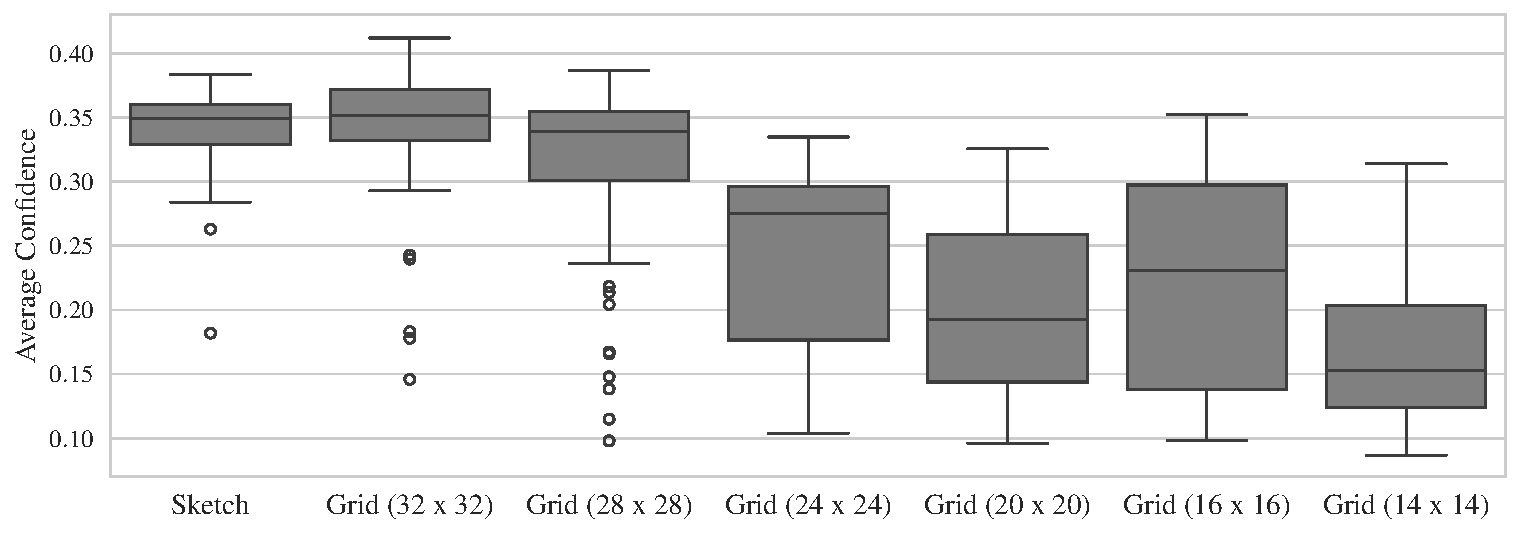
\includegraphics[width=\textwidth]{images/grid_comparison.pdf}
    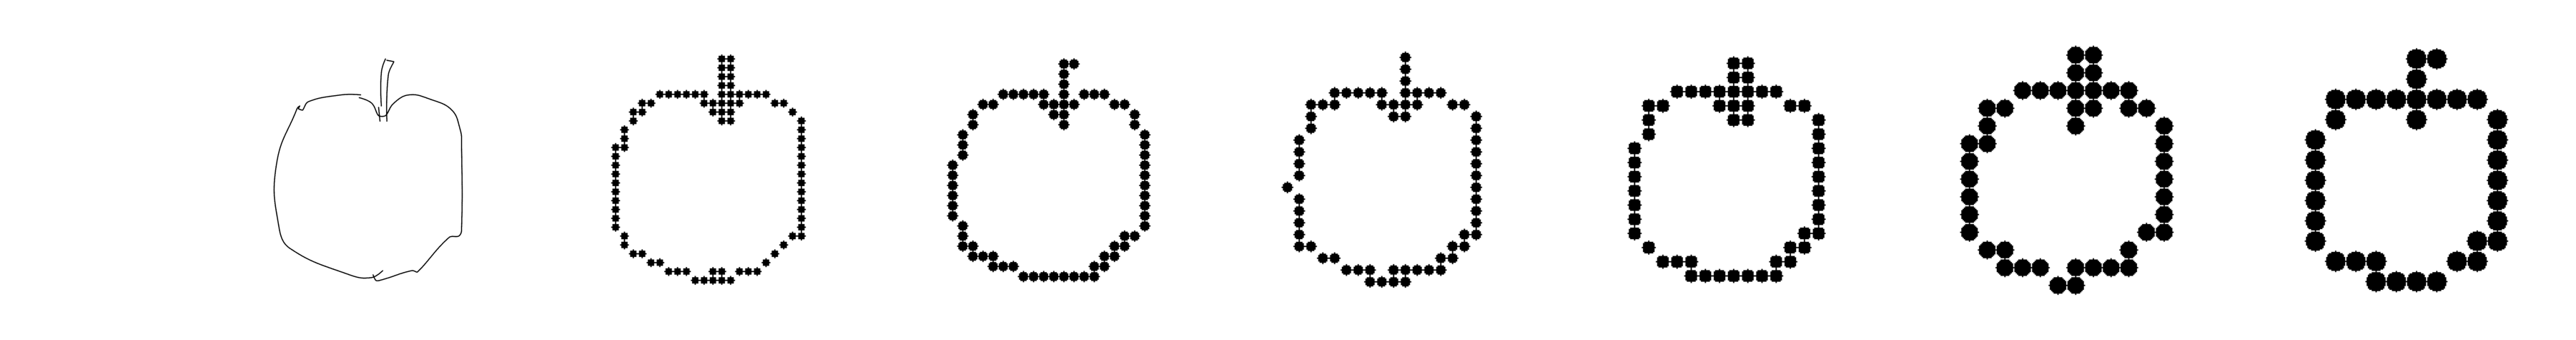
\includegraphics[width=\textwidth]{images/grid_comparison_images.png}
    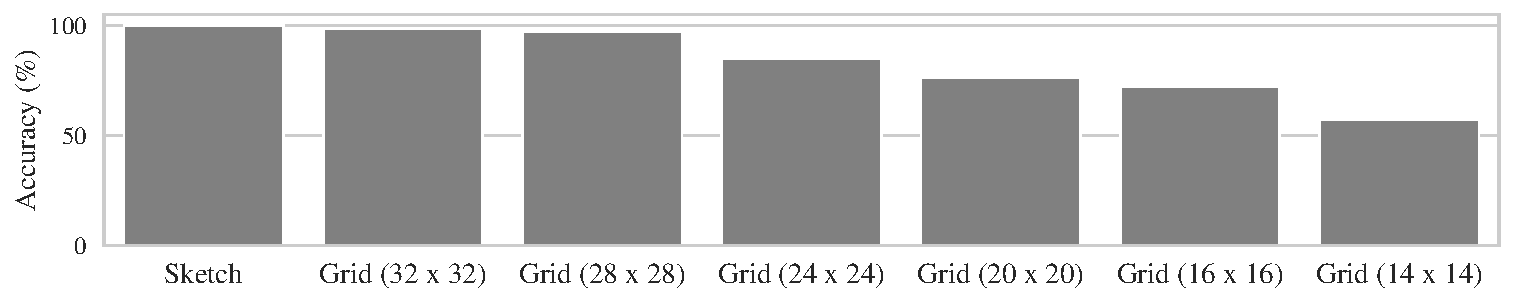
\includegraphics[width=\textwidth]{images/grid_comparison_accuracy.pdf}
    \caption[CLIP on sketches and ShapeGridWorld grids of different resolutions.]{CLIP on sketches and ShapeGridWorld grids of different resolutions.
    The first row shows the comparative similarity of the embeddings of \(80\) sketches of apples (and their grid counterparts) to the label ``sketch of an apple'' using the CLIP variant \texttt{ViT-L/14}.
    The probabilities are calculated using \eqref{eq:clip-dist}, with temperature \(\tau = 1\), to show the trend.
    The categories for this example are ``apple'', ``chair'', ``car'', ``flower'', ``pencil'', ``house'', ``tree'', ``fish'', ``star'', and ``bird''.
    The middle row shows a sample of the images for each of the cases.
    The bottom row shows the accuracy (percentage of correct predictions) for each of the cases.
    }
    \label{fig:clip-sketches}
    % 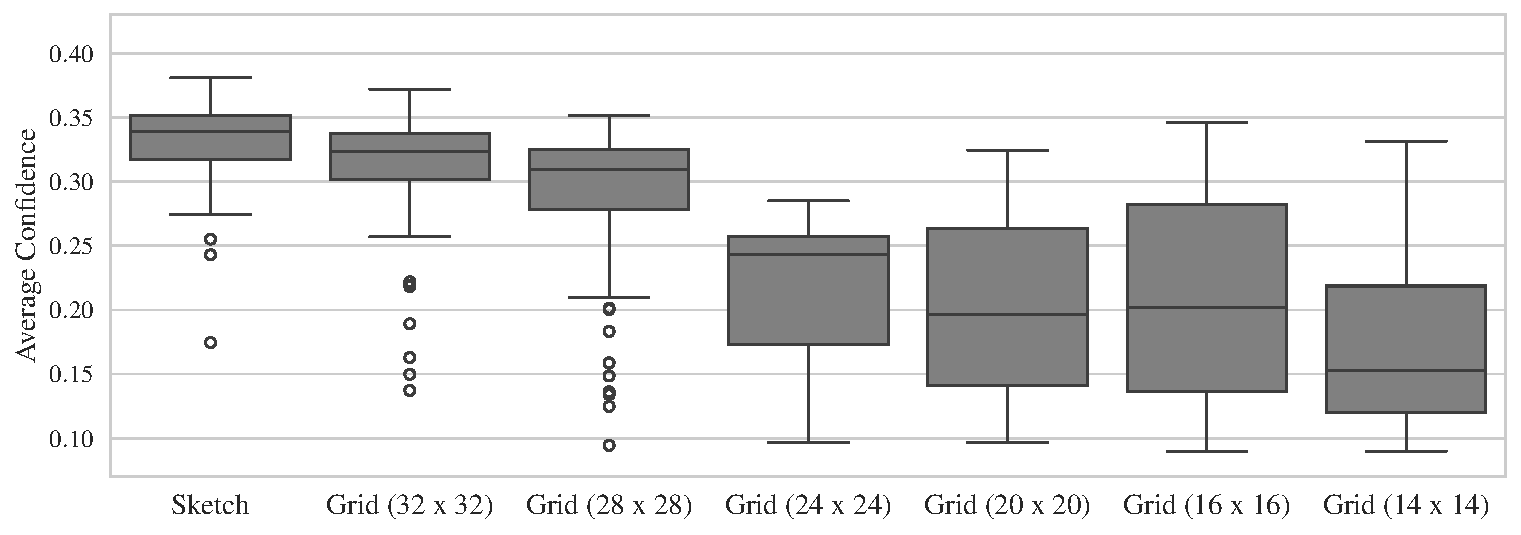
\includegraphics[width=\textwidth]{images/grid_comparison_inverted.pdf}
    % 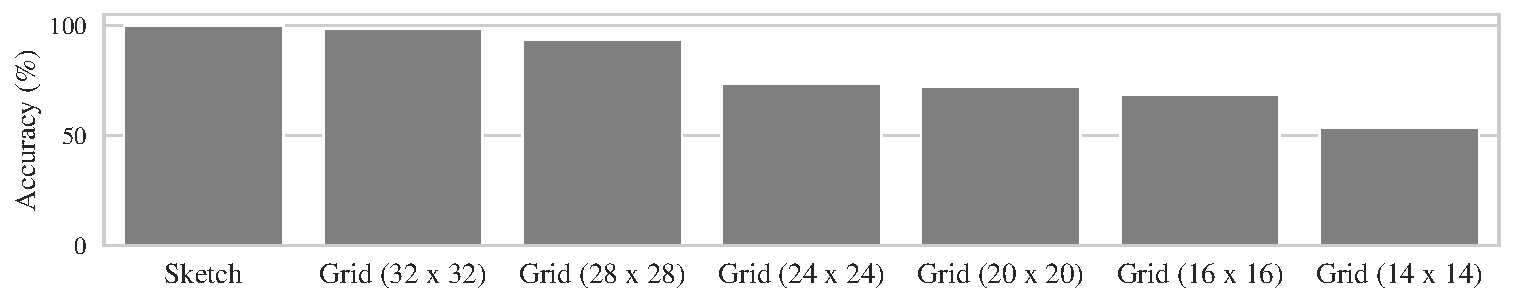
\includegraphics[width=\textwidth]{images/grid_comparison_accuracy_inverted.pdf}
    % \caption{CLIP on \emph{inverted} sketches and ShapeGridWorld grids of different resolutions.}
    % \label{fig:clip-sketches-inv}
\end{figure}
We find that CLIP can recognize these sketches quite well.
As the grid becomes coarser, the confidence and accuracy of CLIP decrease significantly.
For very coarse grids, the accuracy is almost as bad as random guessing.

We also experiment with inverting the images and find that the results are consistently slightly better with black-on-white sketches (shown here) than with white-on-black sketches.
Yet, we do not notice any difference in performance with the addition of grayscale values in the pixel blocks in these experiments.

\newpage
\begin{wrapfigure}[13]{r}{0.39\textwidth}
    \centering
    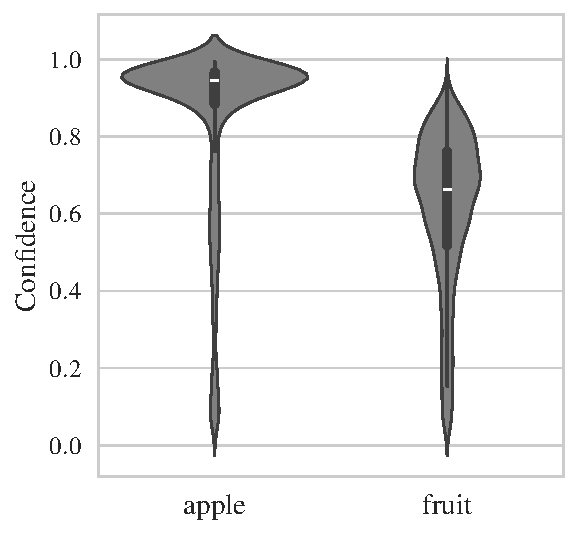
\includegraphics[width=0.36\textwidth]{images/hypercategory_comparison_2.pdf}
    \caption{CLIP on different levels of hypernymy and hyponymy of labels.}
    \label{fig:clip-hypercategory}
\end{wrapfigure}
In most cases, we also notice that using specific labels like ``apple'' for a picture of an apple has better accuracy than using hypernyms like ``fruit'' (\figref{fig:clip-hypercategory}).

Additionally, we find that the bigger CLIP models perform better on these tasks than the smaller ones which is in line with observations from other studies on VLMs as a source of rewards, particularly \cite{vlmrm}.
We tried the same experiments with different sets of categories, prefixes, and suffixes; the results followed similar trends.

\subsection{CLIP on Tangram}
\label{sec:clip-tangram}

Tangram has fewer degrees of freedom than ShapeGridWorld and it is more abstract but it still allows for rich creative expression.
To test if it would be a feasible environment for our study, we test CLIP's accuracy as a zero-shot classifier on some images of creations on Tangram from the internet using classes with simple Tangram arrangements for the text input, \(bfl\).
We again find it to be quite good at recognizing these creations with high confidence.
\figref{fig:clip-tangram} shows a few examples.
\begin{figure}[h]
    \centering
    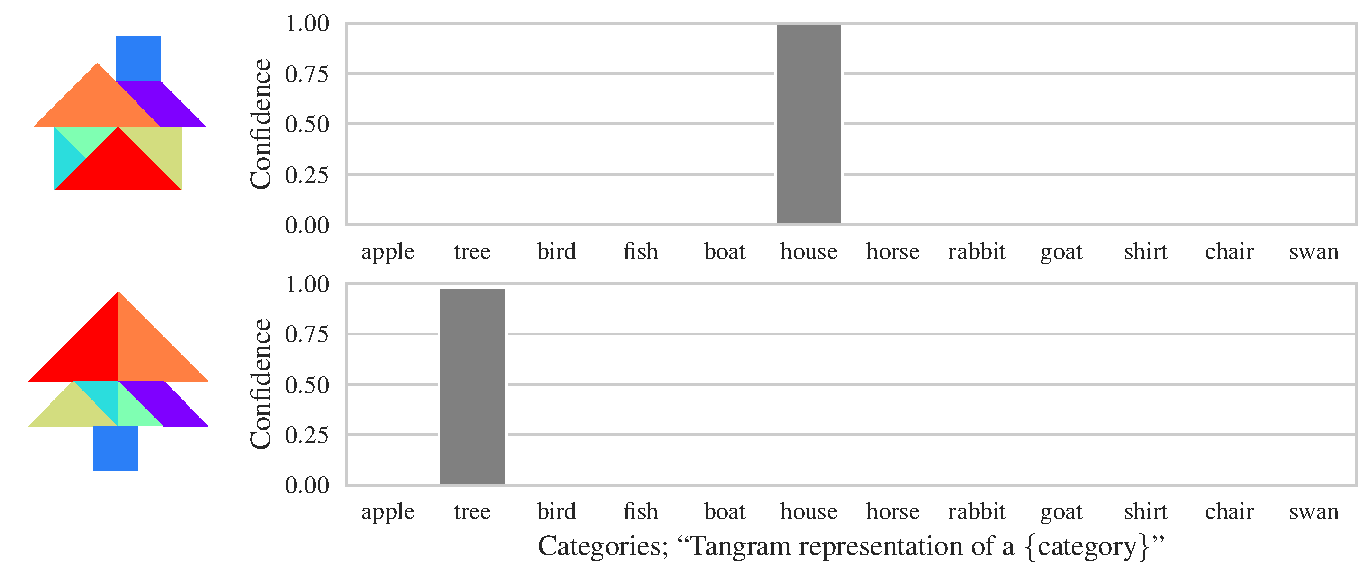
\includegraphics[width=\textwidth]{images/tangram_comparison_10.pdf}
    \caption{CLIP on a few simple Tangram creations.}
    \label{fig:clip-tangram}
\end{figure}

We do not find a significant trend in the effect of colors on the performance of CLIP, but inversions seem to slightly affect the distribution of inferences in certain cases
(one such example is given in \figref{fig:clip-tangram-inversions} in the appendix, where the distribution of CLIP is skewed in grayscale and white-on-black cases).
Consequently, we use both colored and black-on-white binary renderings for our experiments.

More experiments on these hyperparameters are discussed in the later sections.


\section{Trajectory Analysis with Random Rollouts}
\label{sec:clip-problems}
% Problems with CLIP
Although we find that CLIP is good enough at recognizing creations in our environments, we wanted to ensure that it would be a good source of rewards for our environments, or that the controller would be able to exploit it well to reach a sufficiently good local optimum.
To study the semantics entropy reward landscape, we conduct some experiments with \emph{random rollouts} in the environments, i.e. starting from a meaningful creation, we perturb the creation with randomly sampled actions and observe the effects on the reward trajectories.
One such rollout in ShapeGridWorld is shown in \figref{fig:random-rollout}.

\begin{figure}[h]
    \centering
    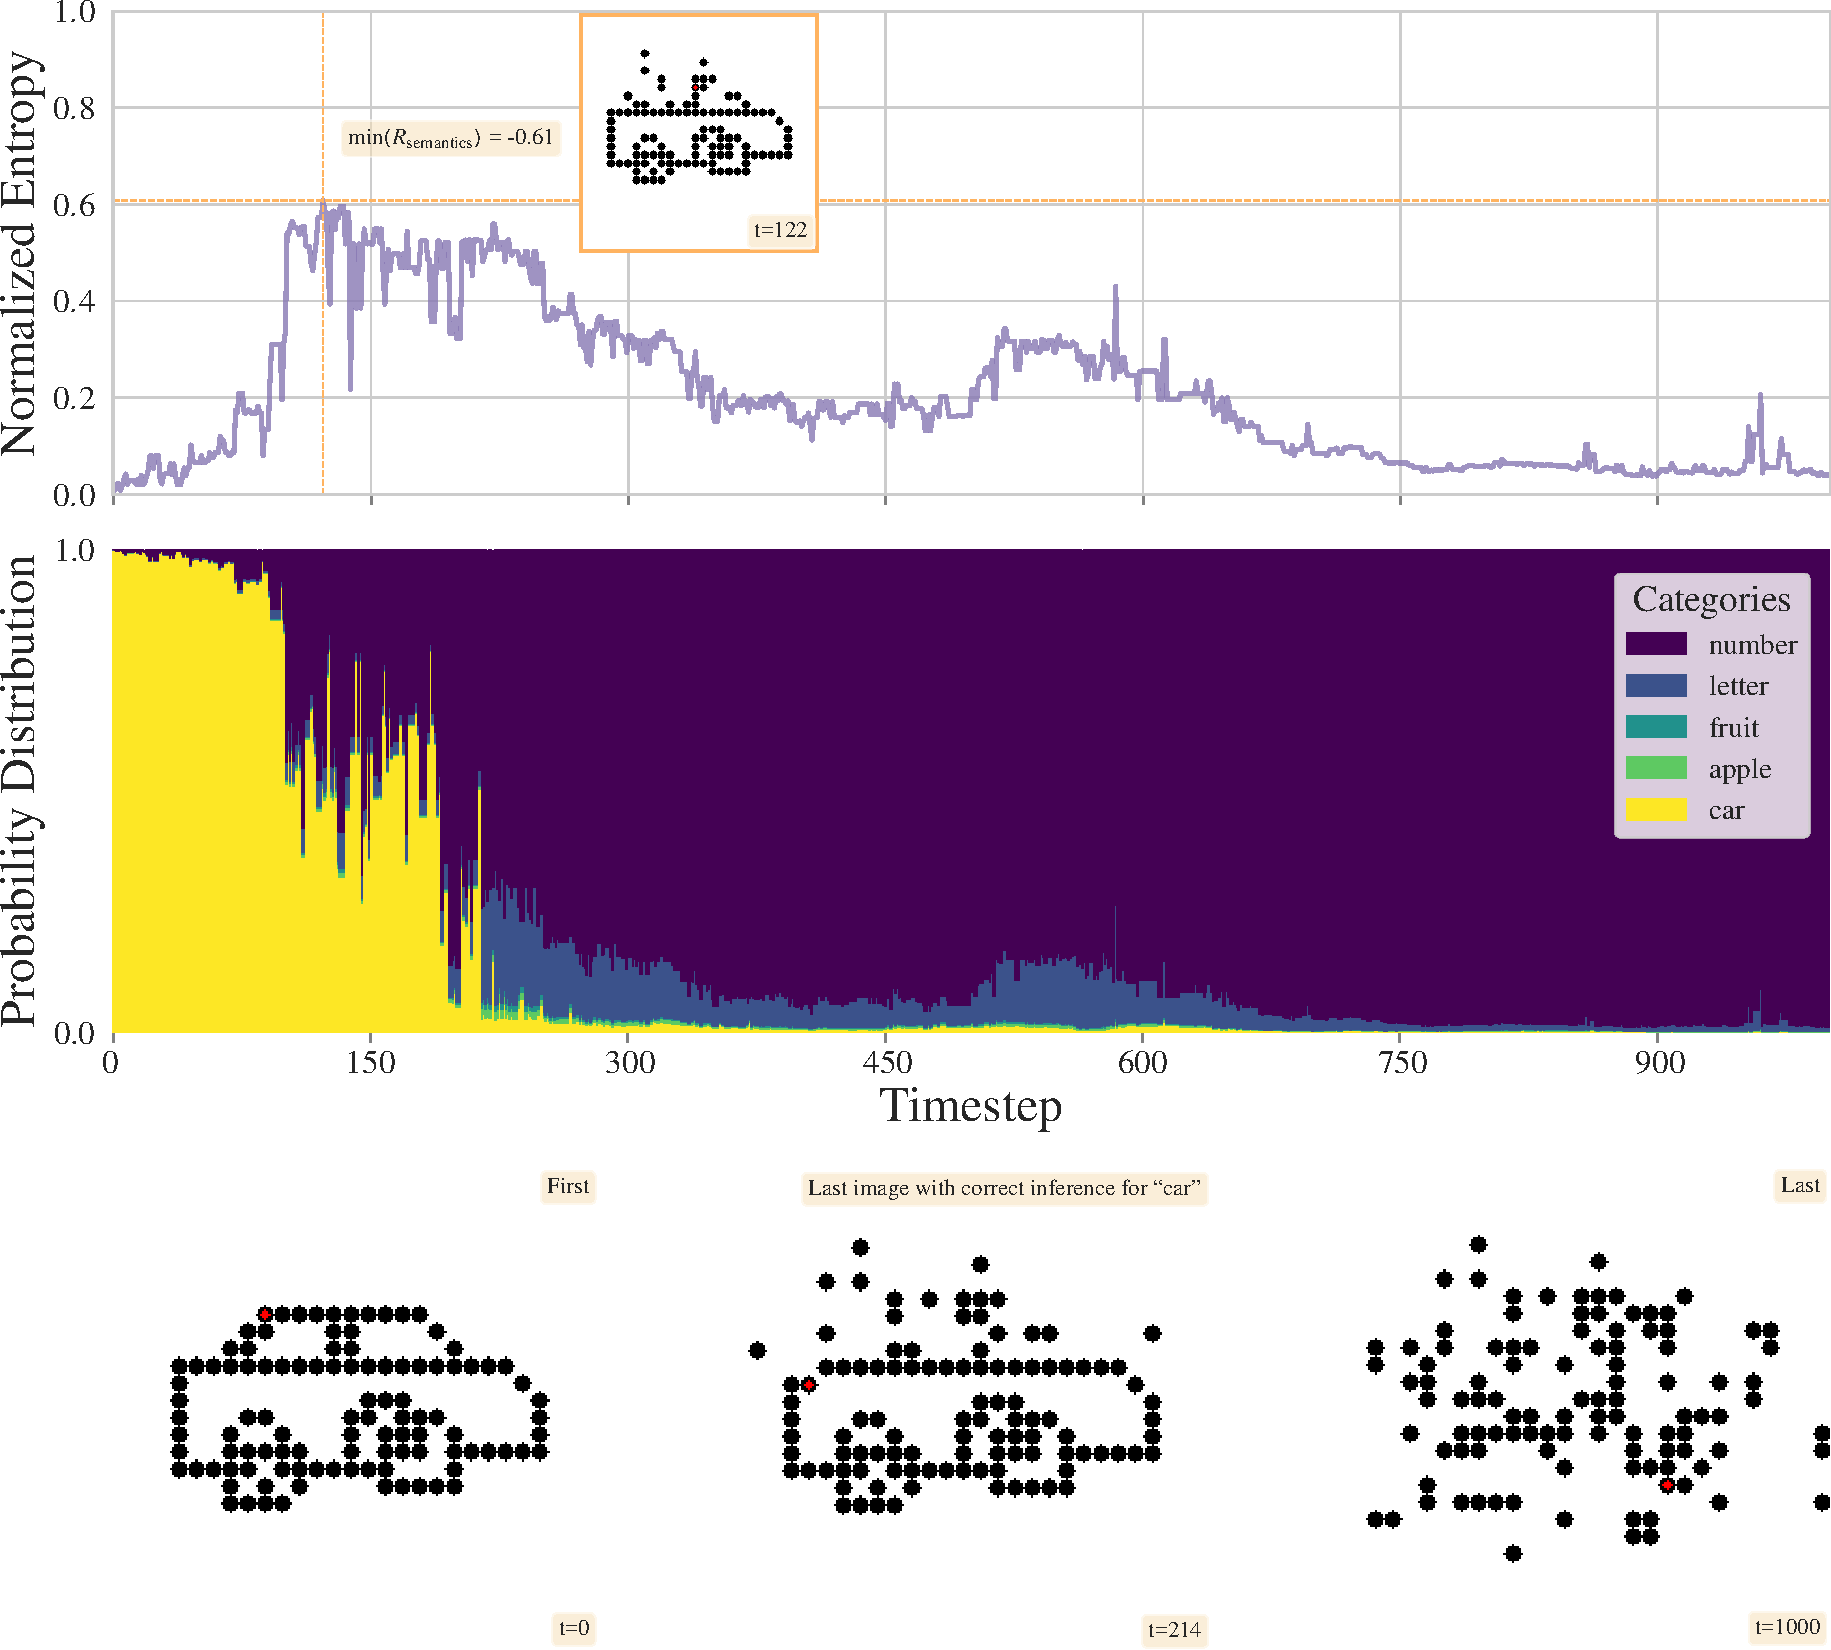
\includegraphics[width=0.8\textwidth]{images/sparse_rewards.pdf}
    \caption[Random rollouts in ShapeGridWorld.]{Random rollouts in ShapeGridWorld. Going from left to right in time, we perturb the grid pixel-by-pixel and observe CLIP's confidence change. The bottom row shows the distribution of CLIP's inferences over the labels ``car'', ``apple'', ``fruit'', ``letter'', and ``number''. The graph in the top row shows the distribution's entropy. The first and last images in the bottom row are the initial and final images respectively.
    The middle image shows the image after which ``car'' is no longer the categorized class.}
    \label{fig:random-rollout}
\end{figure}

These experiments show that CLIP is susceptible to noise in its inferences.
As a consequence of this, the reward is potentially somewhat sparse, and more critically, there is a large semantic bias in not-so-meaningful (random) images.
The following sections discuss each of these problems in detail.

\subsection{Noisy Rewards} % Sudden changes in rewards
\label{sec:noisy-rewards}
We observe that the inference of CLIP breaks suddenly with small changes in the image, i.e. its confidence in its classification is very sensitive and adjusting the position of a single pixel can lead to an abrupt response in the distribution of CLIP's inferences.
This problem is visible in the time range \(\sim 100 - 200\) in \figref{fig:random-rollout}.

This can be interpreted as a jagged reward landscape with many local optima.
This makes the rewards unreliable as they might suddenly change with every little action leading to a lack of continuous incremental feedback towards any goal, potentially stagnating the agent in a state of indecision.
If we imagine this scenario in reverse with an active controller, i.e. when the agent starts from the random image and tries to converge to a meaningful image by relying on the semantics entropy reward, it might register a sudden burst of rewards for small changes in the image, but these rewards could just be artifacts of the noise in CLIP's inferences.
This would make it difficult for the agent to gauge the values of its actions to lead itself to eventual rewards, which in turn might lead to difficult and inefficient learning of action policies.

This demands some regularization techniques that would reduce the noise in CLIP.
This problem is less pronounced in the Tangram environment, but it is still present.
Since we use the iCEM controller which has proved to work well in sparse reward settings, it might show some robustness to this noise, and help mitigate this problem.
It utilizes colored noise to temporally correlate action sequences over the horizon, which could also effectively smooth out the reward landscape.

% Moreover, we typically used the \texttt{sum} cost aggregation function for iCEM to average out the noise in the reward signals over the planning horizon.

\subsection{Semantic Bias in Random Images} % Confidence in random images
\label{sec:inference-noise}
Another consequence of the noise in CLIP we observe from the timesteps after \(\sim 250\) in \figref{fig:random-rollout} is that it confidently classifies random images to a class instead of having a flat distribution, i.e. false positives, as evident here with the class ``number''.

This noisy reward signal can lead the agent to be stuck in plateaued local optima (with a rather meaningless creation that it erroneously finds confident).

The two problems, noisy rewards and semantic bias in random images are not independent.
There is a non-trivial anti-correlation between the two.
That is, increasing reward density (or reducing reward noise) involves increasing confidence in imperfect/partial creations (or adding more semantic bias in random images).


\subsection{Class Preference in CLIP}
\label{sec:class-preference}
Another intertwined issue we face related to the problem of semantic bias in random images is that of class imbalance.
There are some classes in which CLIP is consistently more confident than others and leans towards them over others when unsure.
This includes classes that signify broader concepts such as ``animal'', ``fruit'', ``letter'', ``object'', or ``number'', depending on which is present.
Thus, in free-play, CLIP might converge to these classes more often than others.
% Histograms of the creations we observed in all our simulations together shown in \figref{fig:class-preference-tangram} and \figref{fig:class-preference-sgw} this bias.

% \begin{figure}[H]
%     \centering
%     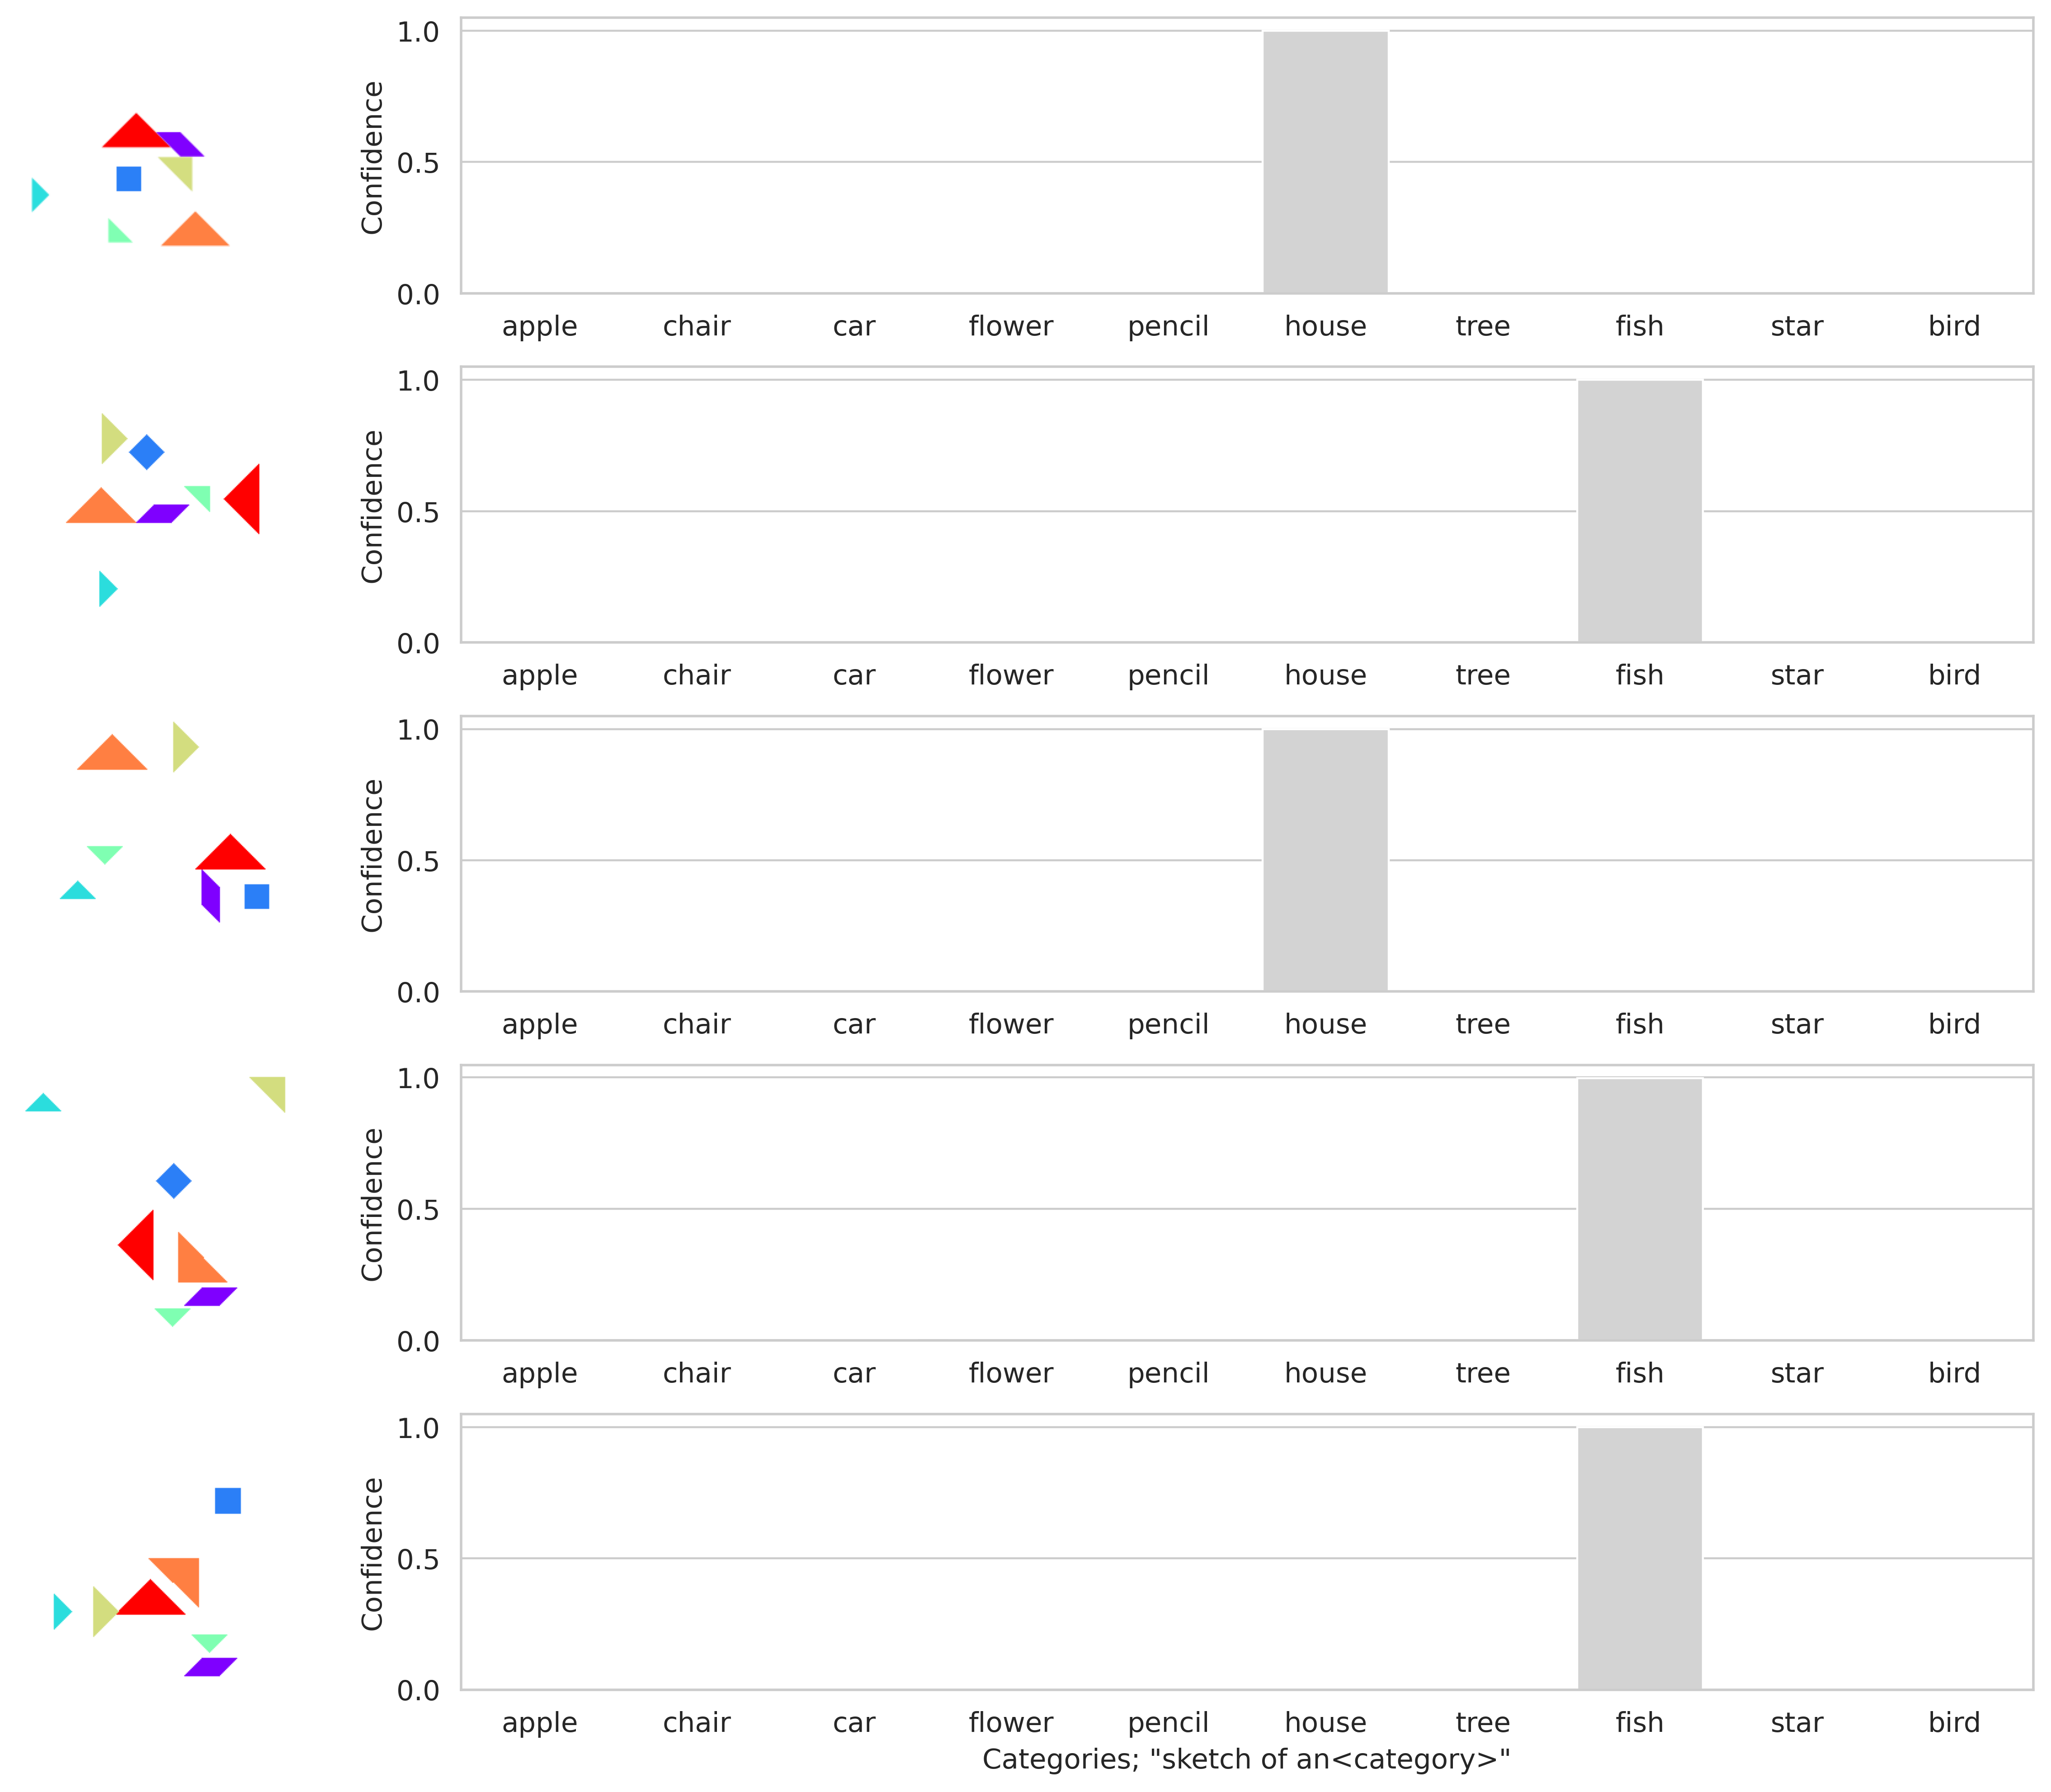
\includegraphics[width=\textwidth]{images/inference_noise.png}
%     \caption{Class preference in CLIP.}
%     \label{fig:class-preference}
% \end{figure}

We can circumvent this issue by avoiding certain classes and choosing enough creative possibilities for the semantics entropy reward such that CLIP's preferences balance out (see \secref{sec:clip-categories}).
Although, this is non-trivial.
Especially for the Tangram environment, in which the creations can be quite abstract, there is only a limited set of semantically distinct, simple, and feasible categories.

% \newpage
\section{Trajectory Analysis with Closeness Costs}
\label{sec:closeness-rollouts}
% closeness_reward_scale
% closeness_reward_threshold
Before we start improving and running simulations using inferences from CLIP, we need to also ensure that the agent could ideally reach a reward-conditioned goal in our environments, i.e. that they are \emph{solvable}, especially for Tangram as it is introduced as a new environment in this study.
Moreover, it is crucial to establish this solvability under sparse rewards.
To ensure that our controller does this efficiently and robustly, a good choice of the iCEM controller hyperparameters and the environment configuration is essential.
These hyperparameters and configurations are dependent on each other so they need to be optimized together.

For example, the size of the grid together with the step size affects the minimum required planning horizon for the controller.
For a small discrete grid or a large enough step size, the planning horizon need not be very high, because the controller can potentially reach the goal in a few steps and does not need to plan far ahead, but on the other hand, if the step size is too small for the grid size, a longer planning horizon is required so that the agent can discover the reward by random sampling of its actions.

In a similar vein, the step size is also related to the ``object persistency'' used in the environments.
This parameter governs how many steps a single object (pixel block in ShapeGridWorld and a polygon in Tangram) is in focus for the actions of the controller before it cycles to the next object in the predefined sequence.
For a high object persistency, the step size could be lower, but for a low object persistency, the step size needs to be higher.

These interdependencies make the hyperparameter optimization problem quite complex and the sheer number of these parameters renders this task very expensive.
Given the high computation resources and time required to run simulations with the semantics entropy reward using CLIP, it is infeasible to do a proper search over all the hyperparameters.
Thus, we instead use an alternative reward function to analyze the effect of the hyperparameters in the Tangram environment.
We call this ersatz reward function the \emph{closeness reward}.

Closeness reward is defined in the context of a fixed target creation in the environment, and it is formulated as the negative of a distance function between the current creation and the target creation in the state space of the environment.

We use two different distance functions, the \emph{dense closeness cost} and \emph{sparse incremental closeness cost}.
The dense closeness cost is formulated as the \(L^2\) distance between the current and target creations and the sparse incremental closeness cost is formulated as the dimension-wise thresholded \(L^1\) distance between the current and target creations, given by,
\begin{equation}
    \label{eq:closeness-reward-sparse}
    \mathit{\Delta}(\bfi, \bft) = \sum_{k \in n_s} \bm{1}_\varepsilon(i_k - t_k),
\end{equation}
where \(\bfi, \bft \in \cS\) are the current and target creations respectively, \(\varepsilon\) is a small threshold, and \(\bm{1}_\varepsilon\) is the indicator function such that \(\bm{1}_\varepsilon(x) = 1\) if \(|x| > \varepsilon\) and \(0\) otherwise.

\figref{fig:closeness-rollouts} shows a sample closeness reward run for the dense closeness cost on the Tangram environment.

\begin{figure}[h]
    \centering
    \href{https://drive.google.com/file/d/15IAo_xsNFSUI0YFVjrIBfn7LAV2hO68E}{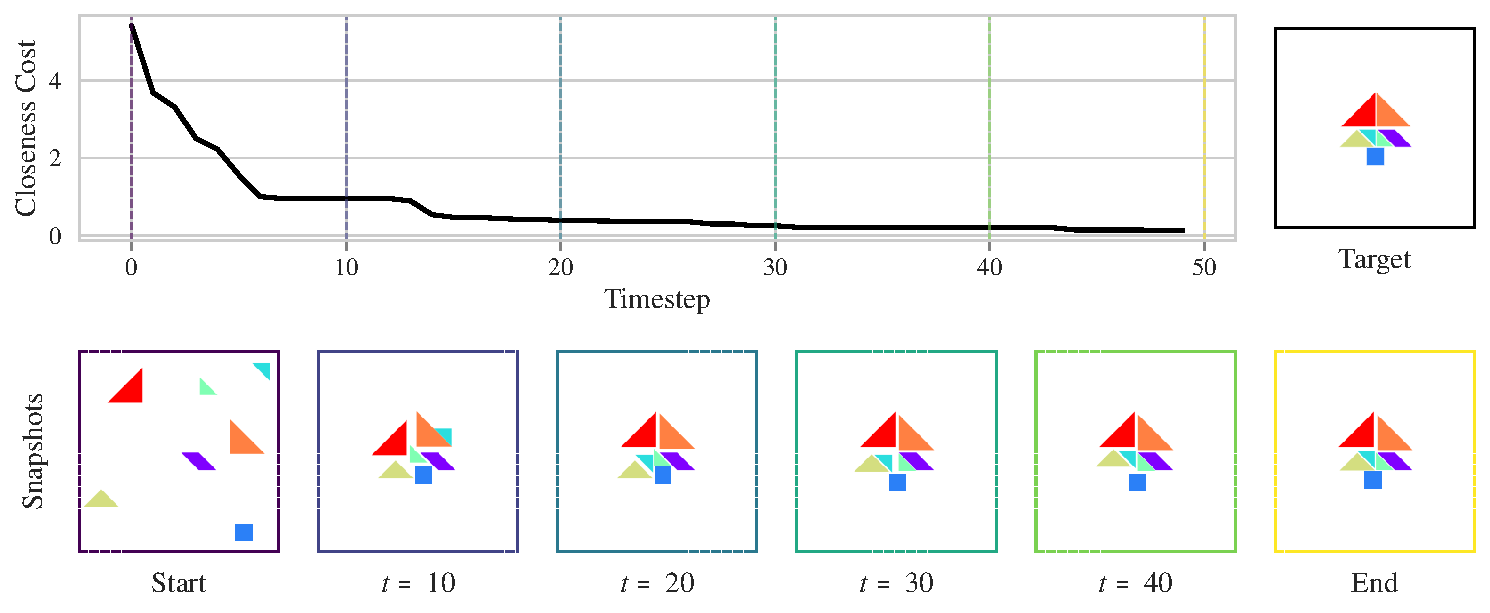
\includegraphics[width=\textwidth]{images/closeness_trajectory_495.pdf}}
    \caption[A successful closeness reward rollout in Tangram.]{A successful closeness reward rollout in Tangram\footnotemark[1].}
    \label{fig:closeness-rollouts}
\end{figure}

Using these closeness reward/cost formulations, we perform an extensive grid search over the many hyperparameters of the iCEM controller and the environment together to find the best combinations and study their effects.
To assess and judge the resulting trajectories and their underlying parameters, we compare their cumulative rewards over the rollouts.

We find that the controller is easily able to achieve the goal under dense closeness rewards for a wide range of hyperparameters and other than a few parameters such as the granularity of the grid, the step size, and the object persistency, we do not notice much difference in the performance of the controller.

The comparison results are only summarised here for brevity. Please refer to the appendix chapters \ref{sec:environments-details} and \ref{sec:icem-details} for more details about these hyperparameters of the iCEM controller and the environments respectively. It also lists the optimal and default values we observed and typically used in our simulations (unless specified otherwise).

Generally, in a continuous Tangram grid, with a step size of \(4\), moving one object at a time for one action step, an iCEM controller with \(128\) trajectories and a minimum planning horizon of \(8\) with \(3\) inner iterations can reach the goal in \(30-60\) timesteps.

The tuning is more demanding under sparse incremental rewards, which requires a higher planning horizon or more sampled trajectories to reach the goal.
This directly corresponds to higher computational costs.

The cost aggregation functions \texttt{best} and \texttt{sum} are comparable in performance and perform better than \texttt{best-\emph{l}}, \texttt{last}, and \texttt{last-\emph{l}}.
With the semantics entropy reward, we expect the \texttt{sum} aggregation function to perform better, due to its summation operation which averages over the rewards in the planning horizon and makes it more robust to noise, essentially having a regularizing effect on the reward landscape.
However, given effective regularization using other methods, the greedier \texttt{best} aggregation function could be more efficient in reaching the goal and escaping local minima.

From this analysis, we gained intuitions about the minimal set of required hyperparameters that allow the controller to solve the environment.
These minimal parameters are later used as a starting point for the simulations with the semantics entropy reward.

\footnotetext[1]{Simulation (with animation) of another similar closeness rollout with a house as the target is available at \url{https://t.ly/jV1dH} or \url{https://drive.google.com/drive/folders/1yGFYLp96O3bEkMu-byQIRGGnOpkvJRcT}.}

% \subsubsection{Tuning Environment Parameters}
% \label{sec:env-hyperparameters}
% % render_kwargs.invert
% % render_kwargs.color

% \label{sec:sgw-hyperparameters}
% % width
% % x_step
% % render_delta
% % object_persistency
% % max_dist
% % control
% % control_boundaries


% \label{sec:tangram-hyperparameters}
% % flip
% % rotate
% % x_size
% % r_size
% % x_step
% % object_persistency
% % max_dist
% % control
% % control_boundaries
% % staging_boundaries


% \subsubsection{Tuning Controller Hyperparameters}
% \label{sec:icem-hyperparameters}
% % action_sampler_params.opt_iterations
% % action_sampler_params.init_std
% % action_sampler_params.elites_size
% % num_simulated_trajectories
% % horizon
% % cost_along_trajectory
% % discount_along_trajectory

% \todo{Talk about the different hyperparameters that were considered. Show histograms of only the significant parameters.}

% \newpage
\section{Improving CLIP Rewards}
\label{sec:improving-rewards}

The regularized semantics reward has some hyperparameters that can be tuned to make the reward landscape smoother.
Namely, the temperature of the softmax function (\(\tau\)), the text baseline regularization strength (\(\alpha_{l}\)), and the image baseline regularization strength (\(\beta_{i}\)).
There are also additional settings such as the categories for the semantics entropy reward, the choice of prefixes and suffixes, the baselines, and the rendering function that can be tweaked to reduce the noise in the reward landscape.

The complex nature of the reward landscape and the high dimensionality of the search space make it difficult to analyze the effects of these hyperparameters.
In this section, we try to gain an intuition over them and reduce the search space.
For this purpose, we use the best of the previous rollouts with the closeness reward from \secref{sec:closeness-rollouts} and run post hoc inferences on the resulting sequence of image observations using CLIP to calculate the trajectories of the resulting \emph{indirect} semantics entropy reward.\footnote{The large number of combinations due to the high dimensional space makes it infeasible to show the subtleties of the interplay between the different hyperparameters in a few figures.
Thus, we have additionally made the analysis available for the reader as an interactive notebook at \url{https://colab.research.google.com/drive/1UzKb5t5PDRO05GbSKpgzWd3DELfAzDxJ} or \url{https://t.ly/j84on}, where one can pick a combination of different hyperparameters to see their combined effects.}
% In this section, we show the results of our experiment with these parameters and additionally test the efficacy of several other methods such as the use of negative embeddings, the addition of post-suffixes, and tweaking the rendering function (adding texturing or modifying the images with other operations) in reducing the noise from CLIP.

\subsection{Effect of Prefix and Suffix}
\label{sec:prefix-suffix}

Given a generic set of simple Tangram creations for the creative possibilities, we find that the choice of prefix and suffix can affect the reward trajectories in unexpected ways. \figref{fig:prefix-suffix} compares the performance for some combinations.
Performance here is measured in terms of the mean-shifted cumulative rewards.

\begin{figure}[h]
    \centering
    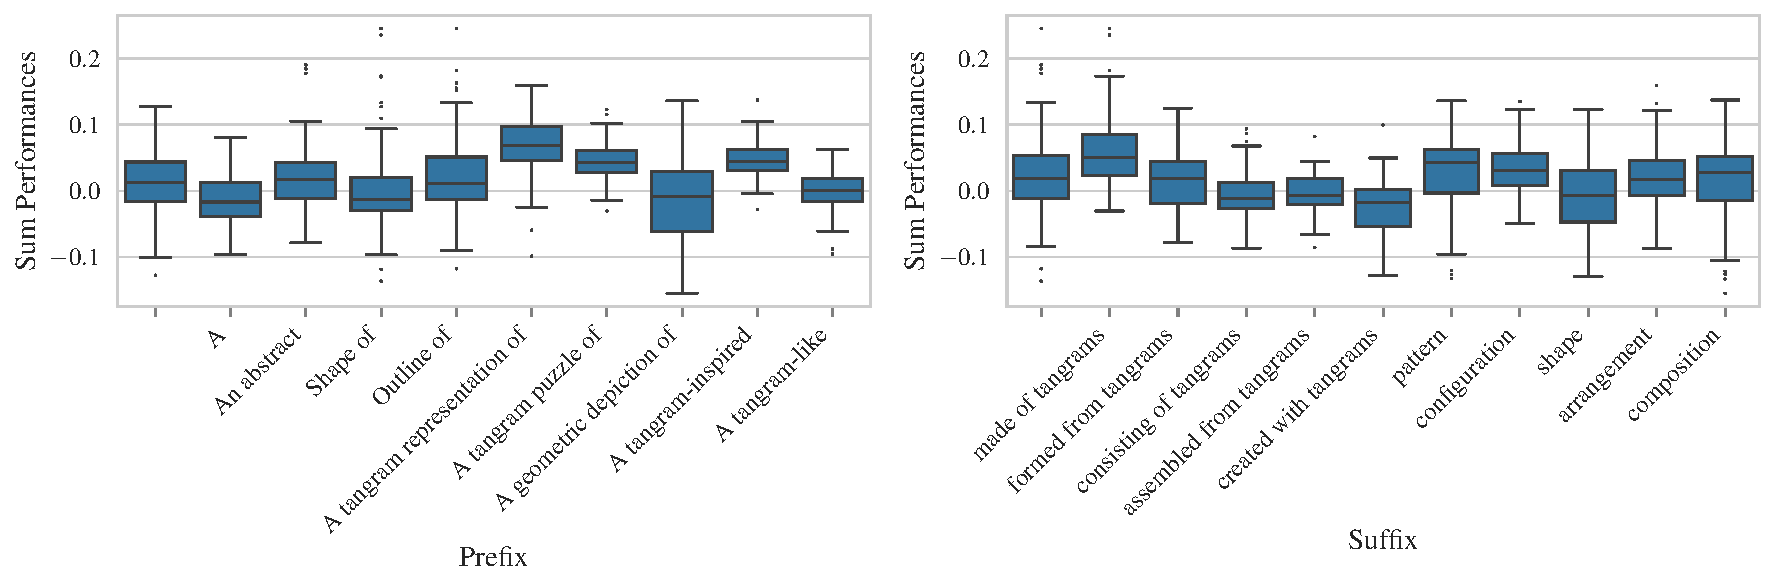
\includegraphics[width=\textwidth]{images/prefix-suffix.pdf}
    \caption{Effect of prefixes and suffixes on semantics entropy reward trajectories in Tangram.}
    \label{fig:prefix-suffix}
\end{figure}
\vspace{-7pt}

Consequently, to capture the underlying trends and find robust values that are agnostic to such prompt engineering in the other parameters discussed next, we analyze and compare their effects over multiple choices and combinations of these prefix-suffix pairs.

This analysis shows some clear trends in the effects of these hyperparameters on the reward landscape which we present in independent ablation studies in the following sections.
Unless specified otherwise, we chose the best-performing values of hyperparameters not under consideration in that section.

To demonstrate the effects, we plot the costs and cumulative semantics entropy costs as a measure of performance.
Ideally, lower cumulative costs indicate better performance, but it has to be interpreted with caution due to the subjective nature of the goal here (semantic expression). Even with a higher cumulative cost, the agent can reach a more semantically expressive state.
We discuss these results, caveats, and effects accordingly in prose.

Additionally, note that in the trajectory plots such as \figref{fig:clip-temperature}, the costs are filtered with a moving average filter of length \(3\) to reduce clutter and make the trends more visible.
The original unfiltered mean trajectories are underlaid in the same plot but in fainter colors.

% The results in this section can be compared to the corresponding adversarial study results discussed in \secref{sec:adversarial-performance}.

% \newpage
\subsection{Effect of the Number of Creative Possibilities}
\label{sec:clip-categories}
To alleviate the problem of class preference in CLIP, we experiment with many combinations of different numbers of categories.
\figref{fig:clip-categories} shows its effect on the entropy of CLIP inferences on a random image.

\begin{figure}[H]
    \centering
    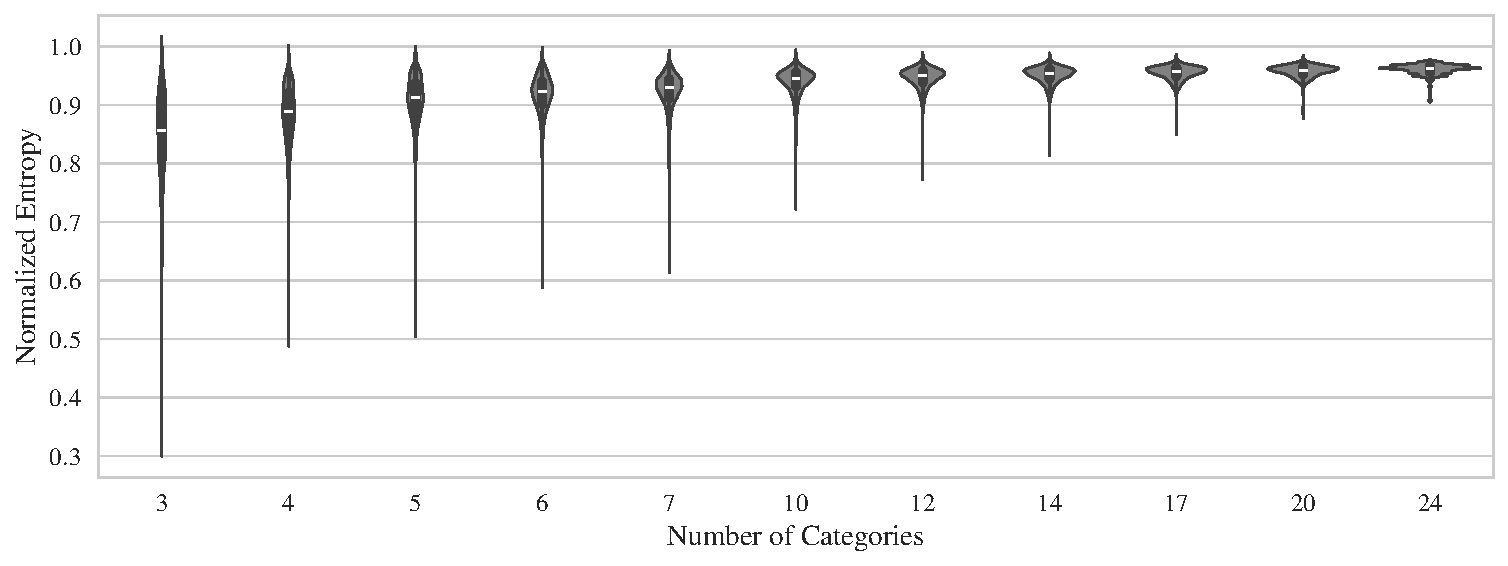
\includegraphics[width=\textwidth]{images/category_comparison_tangram.pdf}
    \caption{Effect of the number of categories on CLIP inference distribution over a random image.}
    \label{fig:clip-categories}
\end{figure}
\vspace{-7pt}
We observe that too few categories can promote semantic bias and class preference in random images as they can have low entropies. Yet, too many categories can exacerbate the problem of noisy rewards since there are potentially more misleading distractions for the agent.
This suggests that a moderate number of categories would be optimal.
For our simulations, we typically choose a set of \(10 \sim 20\) categories with simple Tangram patterns like ``house'', ``bird'', ``boat'', or ``fish'', and avoid broad categories like ``number'' or ``letter'' to circumvent the problem with class preference (see \secref{sec:semantics-entropy-reward-details} for the complete list).
For SGW, we extensively experiment with different sets (see \secref{sec:sgw-categories} for results).

% Additionally, it is important to choose categories that are not too broad to avoid the problem of semantic bias in random images.

\subsection{Effect of Temperature}
\label{sec:reg-temperature}
% semantics_model_temperature

Temperature is a crucial hyperparameter for the softmax function in the semantics entropy reward as it directly controls the entropy of the CLIP distribution (see \eqref{eq:clip-dist}).
\figref{fig:clip-temperature} shows its effect, averaged over multiple choice of prefixes and suffixes.
The original CLIP publication recommends a temperature of \(0.01\) for most use cases, which we also find to most often work best to reach a good optimum.
Temperatures up to \(0.02\) are good as well but any value below this range performs significantly worse as it adds to the noise of CLIP, and any temperature above this range renders the reward landscape too smooth and the reward trajectories too flat, leading to a loss of any semantic bias from CLIP.
% This is a post hoc CLIP inference on trajectory samples from the closeness reward rollout experiments.

\begin{figure}[H]
    \centering
    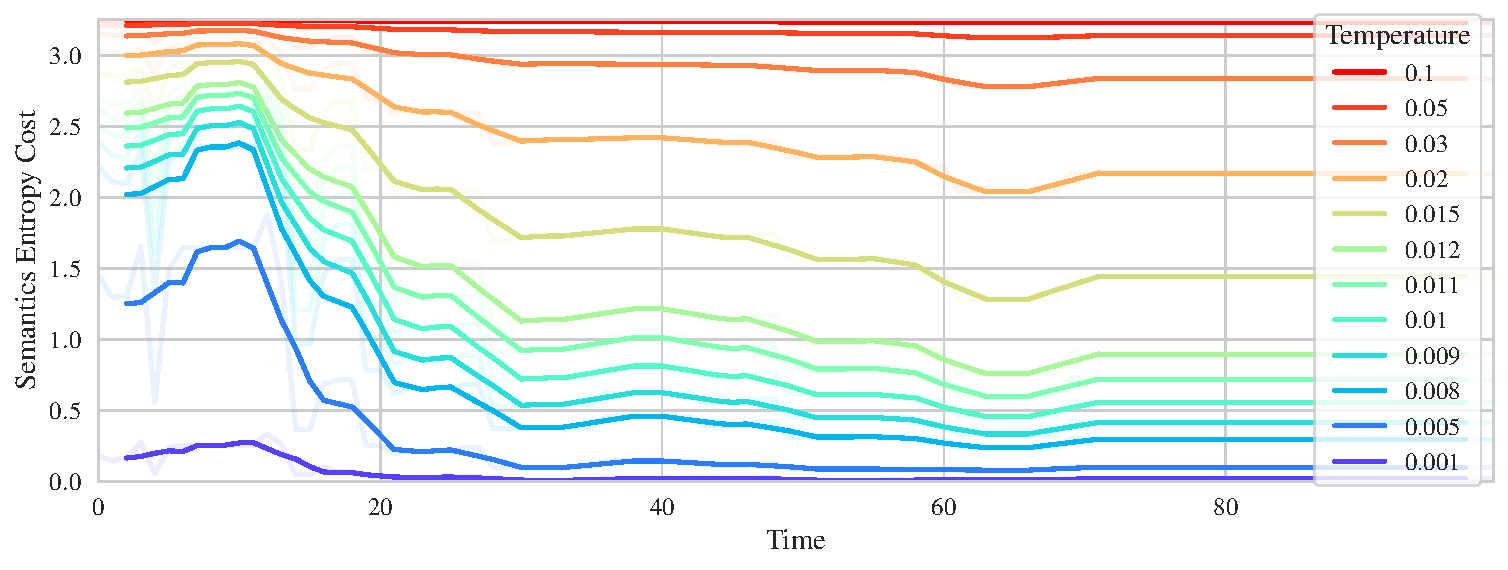
\includegraphics[width=\textwidth]{images/temperature_comparison.pdf}
    \caption{Effect of temperature on semantics entropy reward trajectories.}
    \label{fig:clip-temperature}    
\end{figure}

\subsection{Effect of Baseline Regularization}
\label{sec:reg-alpha-beta}
% semantics_alpha_target

The regularization strengths of the text baseline (\(\alpha_{l}\)) and the image baseline (\(\beta_{i}\)) are arguably the most important hyperparameters for the regularized semantics entropy reward.
Baseline regularization helps by providing better directional guidance in the CLIP embedding space.

We compare the cumulative semantics entropy rewards of the post hoc inferences on closeness reward trajectories with different values of \(\alpha_{l}\) and \(\beta_{i}\) to find the optimal values and find the best values of the regularization strengths to be somewhere in the middle of the two extremes, with the optimal image baseline regularization strength slightly higher than the text baseline regularization strength.
This is in line with the findings of \cite{vlmrm} in goal-conditioned reward settings.

\figref{fig:clip-alpha-beta} shows these results, averaged over multiple choice of prefixes and suffixes.

\begin{figure}[H]
    \centering
    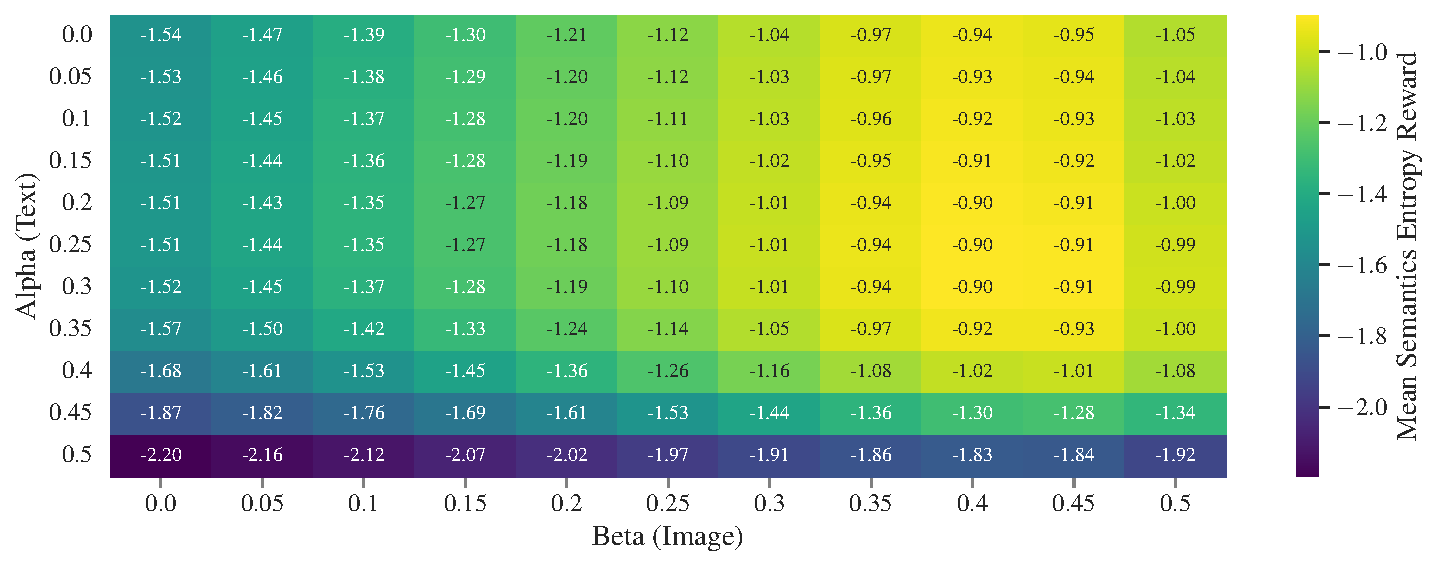
\includegraphics[width=\textwidth]{images/alpha_beta_temp12avg_noneg.pdf}
    \caption{Effect of regularization strength on semantics entropy reward trajectories.}
    \label{fig:clip-alpha-beta}
\end{figure}

% , like ``house'', ``tree'', ``bird'', ``goat'', ``shirt'', ``swan'', ``goose'', ``teapot'', ``gun'', ``apple'', ``car'', ``airplane'', ``guitar'', and ``flower''

% \subsection{Effect of Changing Prefix and Suffix}
% \label{sec:prefix-suffix}
% % label_prefix
% % label_suffix
% Different prefixes/suffixes and combinations of them also affected the performance of CLIP.

% \begin{figure}[H]
%     \centering
%     \missingfigure{Effect of changing the prefix suffix.}
%     \caption{Effect of different prefixes and suffixes.}
%     \label{fig:prefix-suffix}
% \end{figure}

\subsection{Effect of Negative Embeddings}
\label{sec:negative-embeddings}
\cite{negprompt} used negative embeddings as target baselines in their goal-conditioned CLIP reward function to make the reward landscape smoother.
We experiment with this as well, and instead of using the initial description of the environment as the text baseline, we use a negative formulation of this description.

Yet, we do not find this to be helpful in our experiments.
Instead, it seems to flatten the reward landscape (see \figref{fig:baseline}).
We think this is a consequence of CLIP's language encoder being a bag-of-words model, which makes the negative embeddings essentially close to the target embeddings, and effectively zeros them out.

\begin{figure}[h]
    \centering
    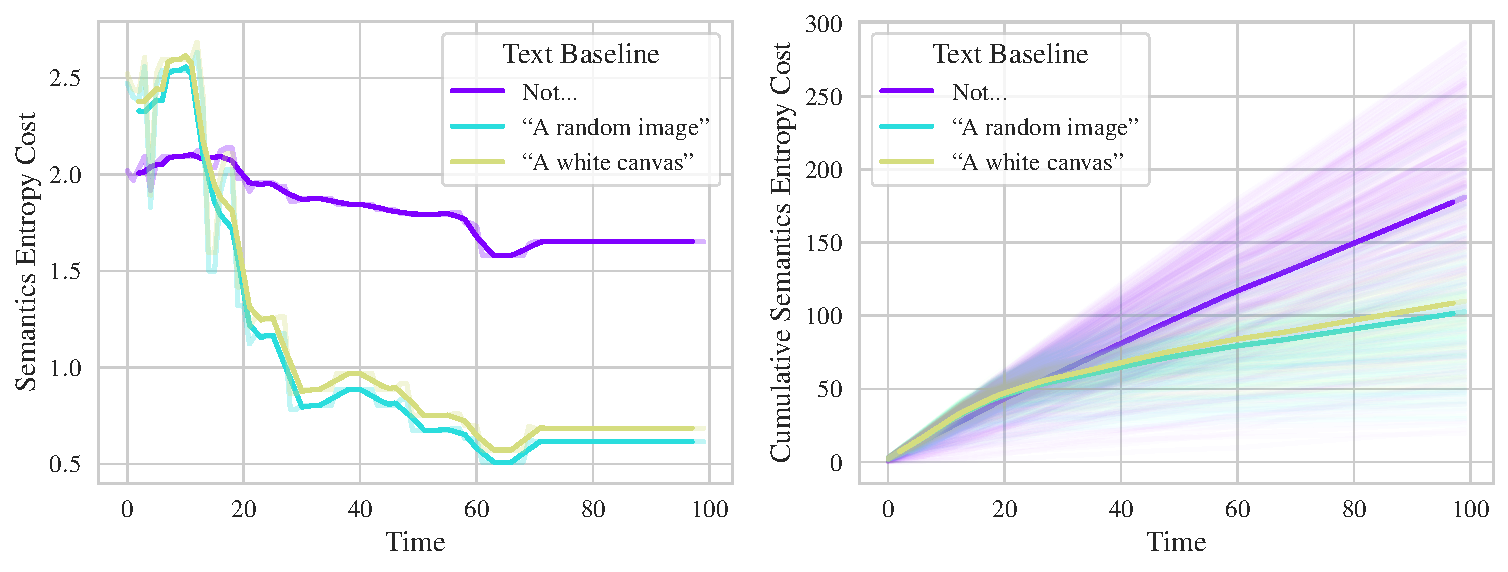
\includegraphics[width=\textwidth]{images/baseline_comparison.pdf}
    \caption{Effect of different text baselines on semantics entropy reward trajectories.}
    \label{fig:baseline}
\end{figure}

\subsection{Effect of Adding Post-Suffix}
\label{sec:post-suffix}
\cite{waffleclip} found that adding a concept and \emph{post-}suffix to the label in the text input to CLIP improved the quality of the inferences.
This post-suffix can even consist of a random string of characters, and by itself also improves the quality of the inferences, albeit slightly.

Following these insights, we also experiment with adding random jibberish to the end of the label as a post-suffix but do not find it to affect the reward.
\figref{fig:post-suffix} shows the effect of different post-suffixes on the semantics entropy reward trajectories, averaged over combinations of prefixes and suffixes.

\begin{figure}[H]
    \centering
    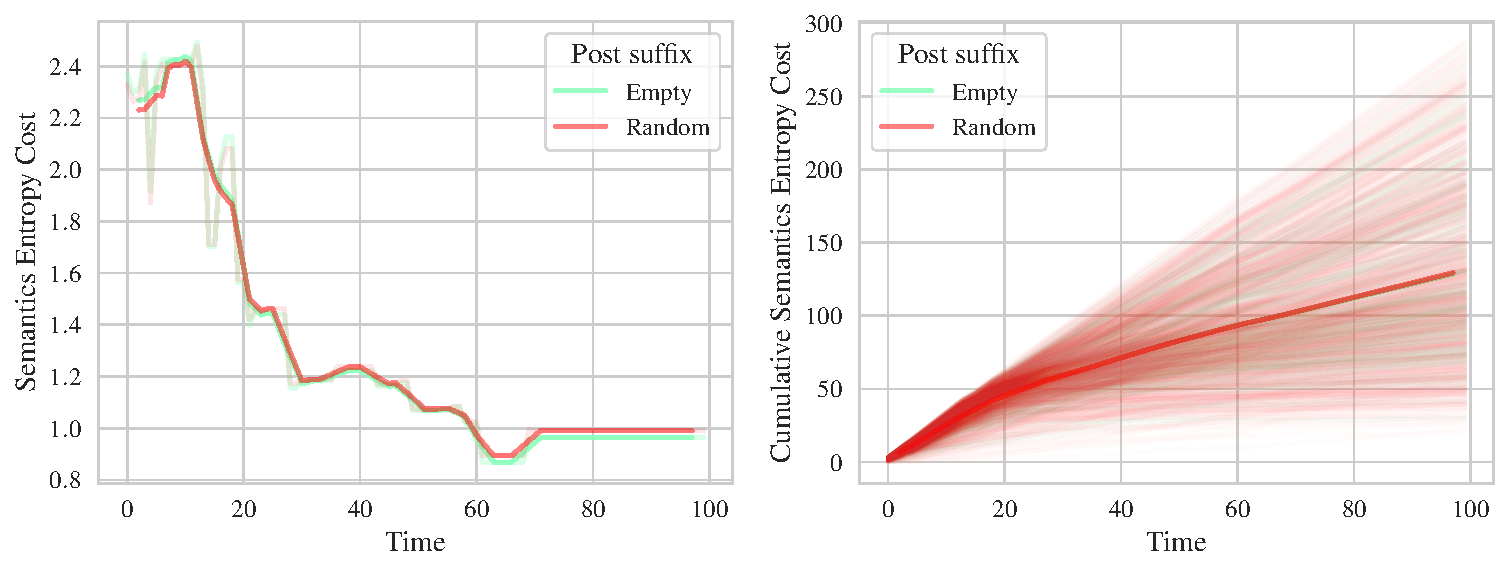
\includegraphics[width=\textwidth]{images/post_suffix_comparison.pdf}
    \caption{Effect of different post-suffixes on semantics entropy reward trajectories.}
    \label{fig:post-suffix}
\end{figure}

% \begin{figure}[H]
%     \centering
%     \missingfigure{As a consolidation of everything before, a bar plot with ablations.}
%     \caption{Ablations of the different methods to improve semantics entropy reward.}
%     \label{fig:clip-ablation}
% \end{figure}

% \newpage
\subsection{Entropy Regularization}
\label{sec:entropy-regularization}
Another promising way to make the reward landscape of CLIP smoother is to fine-tune it with an additional entropy regularization loss over its output.
This is given by,
\begin{equation}
    \label{eq:entropy-regularization}
    L(\bmi, \bml) = L_{\iota}(\bmi, \bml) \underbrace{+ \kappa \sum_{\bfi_k \in \bmi}\sum_{\bfl_j \in \bml} P(\bfl_j; \bfi_k, \bml) \log P(\bfl_j; \bfi_k, \bml)}_{\text{Entropy Regularization}},\\
\end{equation}
where \(L_{\iota}\) is the contrastive cosine-similarity loss used to train CLIP, $\kappa$ is the regularization strength, and \(P(\bfi_k, \bml)\) is the classification probability distribution of image \(\bfi_k\) over the labels \(\bml\) predicted by CLIP.

We experiment with this regularization method to train toy convolutional neural networks (CNNs) for classifying handwritten digits from the MNIST dataset \citep{mnist}, which we call \emph{flatnet}.
Furthermore, we augment the training dataset with varying sizes of random-image samples labeled with a uniform distribution over the categories and train multiple networks.

We find the preliminary results to be quite effective in reducing the noise of the model; it seems to relieve both of the problems from \secref{sec:clip-problems} -- the reward trajectory is smoother, and there is less semantic bias in random images and even less class preference for random inputs.

Yet, we do not use it to fine-tune CLIP to constrain the scope of the project given the limited time.
More information on this analysis can be found in Chapter \ref{sec:flatnet} of the appendix.

% \newpage
\subsection{Adversarial Performance}
\label{sec:adversarial-performance}
To especially tackle the problem of semantic bias in random images, we collect samples of the false positive image observations from our rollouts, called \emph{adversarial observations} (\figref{fig:semantic-bias-random}), by filtering out the image observations with low entropy from all our runs and then manually removing the ones that are true positives.

\begin{figure}[h]
    \centering
    % \includegraphics[width=0.6\textwidth]{images/p_random_semantic_bias.png}
    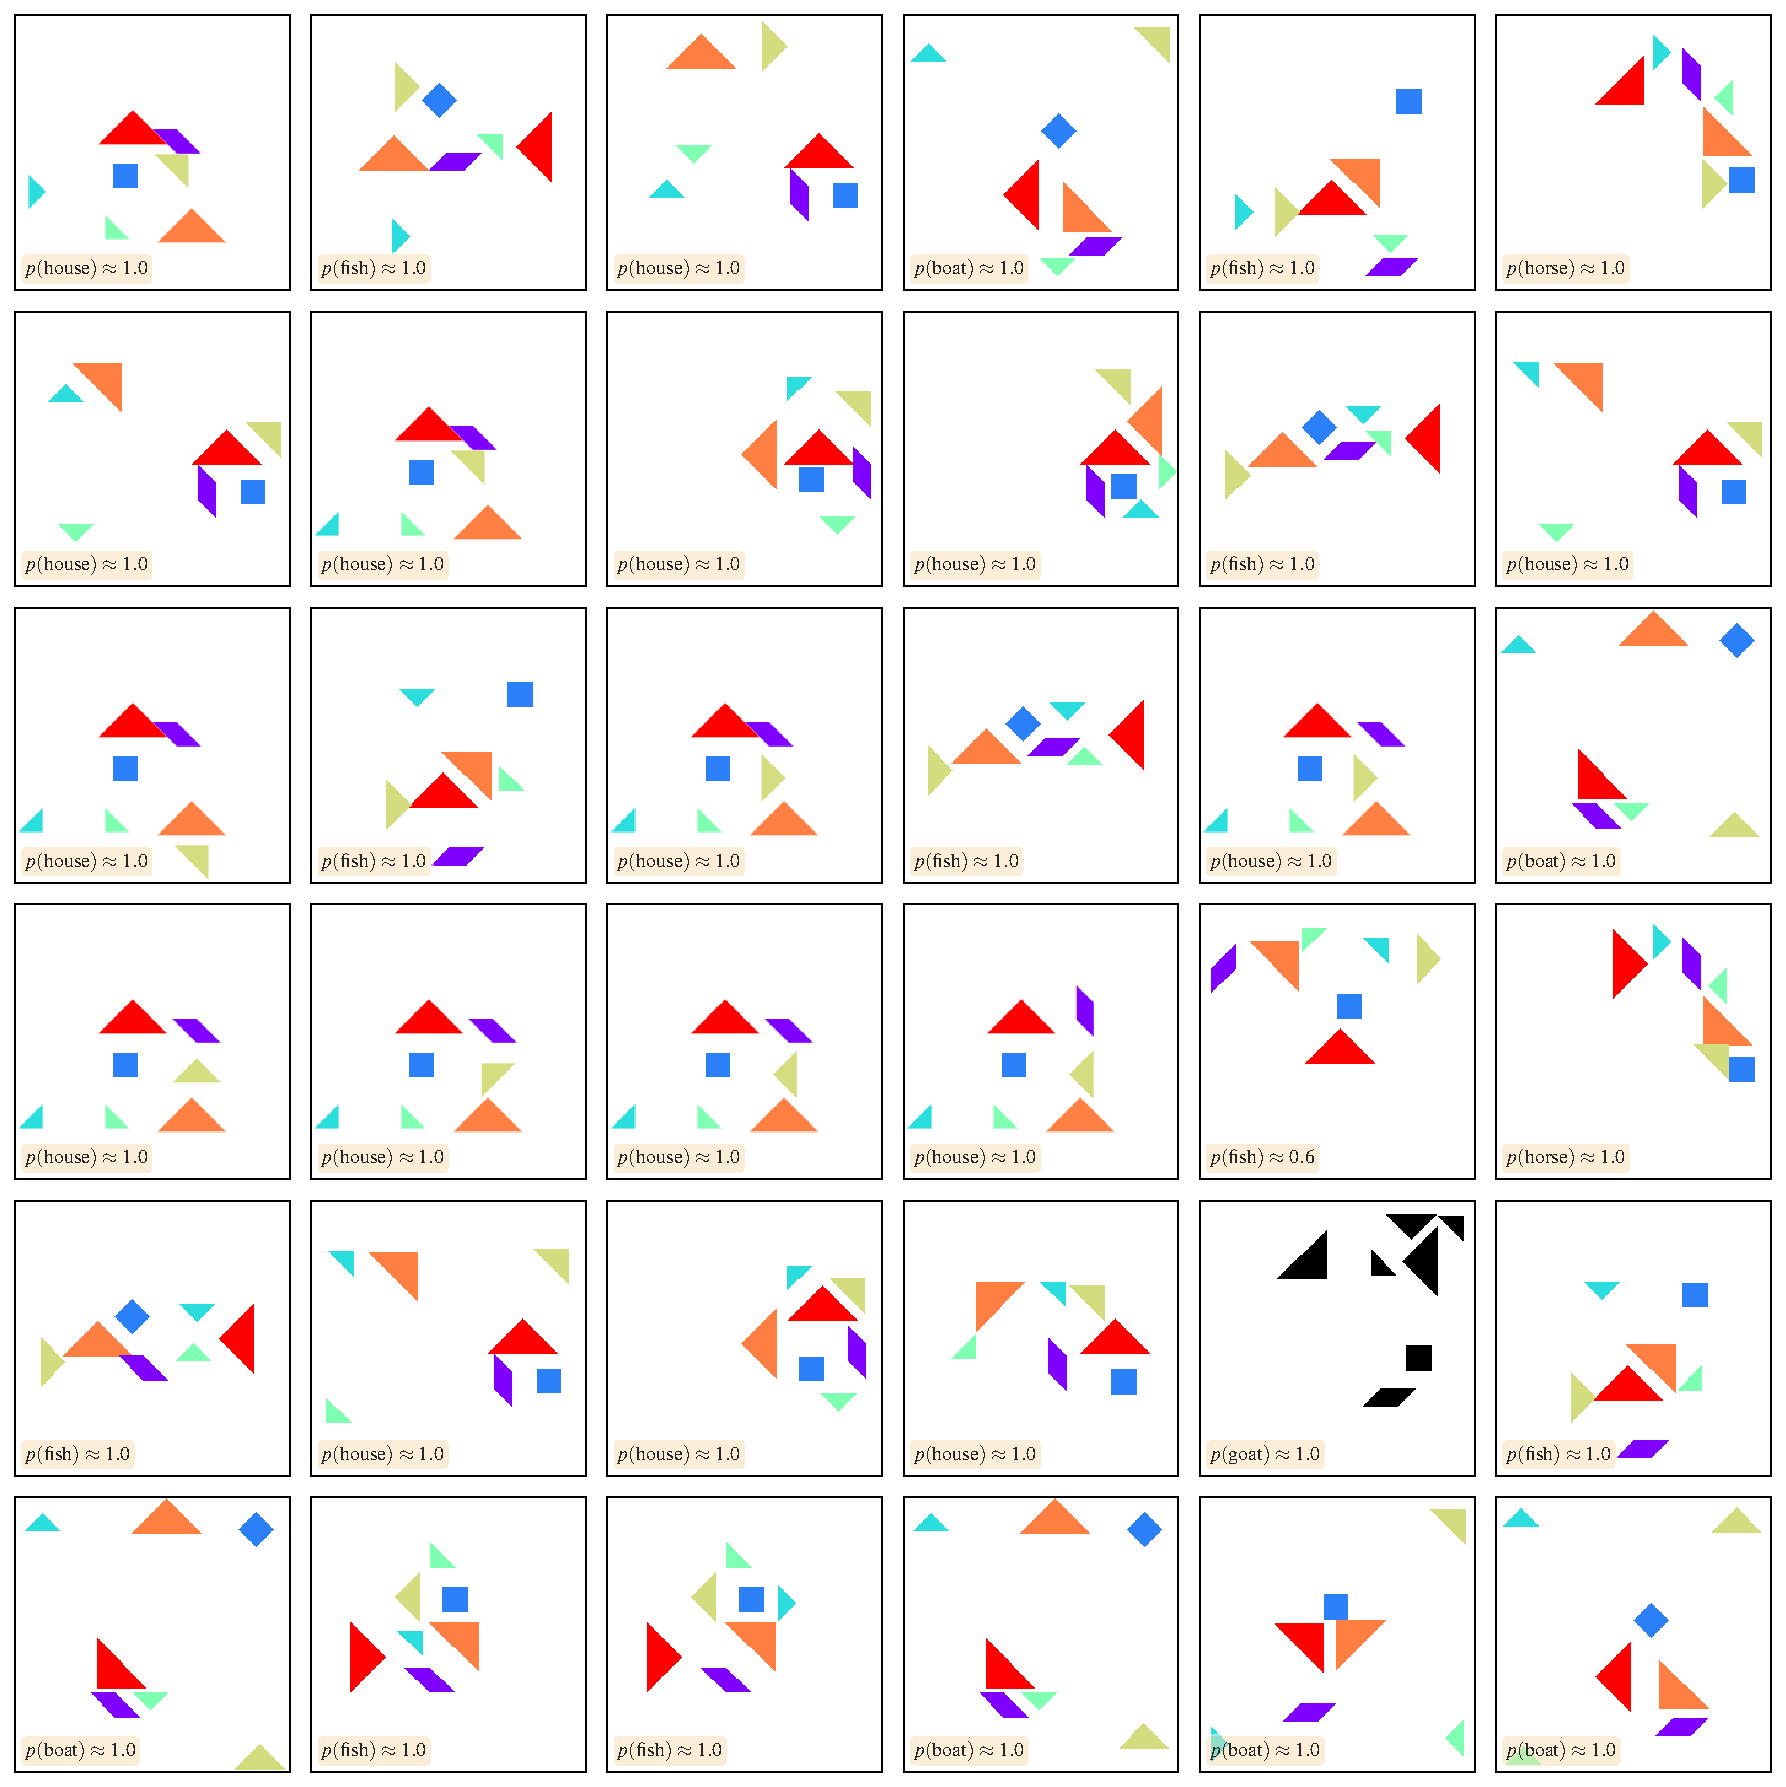
\includegraphics[width=\textwidth]{images/adversarial_samples.pdf}
    \caption{Adversarial samples from simulations.}
    \label{fig:semantic-bias-random}
\end{figure}

Then, we search for the semantics reward regularization hyperparameters that make CLIP less confident in the adversarial images while maintaining its inference for the truly semantically expressive images, i.e. increases its specificity while maintaining its sensitivity.

In this analysis, we use the mean entropies of the false positive and true positive images as our metrics to gauge the performance improvements.
\figref{fig:clip-temperature-adversarial} to \ref{fig:post-suffix-adversarial} show the effect of temperature, regularization, negative embeddings, and post-suffixes on discerning true positives from false positives, over a range of prefix-suffix combinations.

The results from these can be compared to the corresponding results shown before in \secref{sec:reg-temperature} to \ref{sec:post-suffix}.

\begin{figure}[H]
    \centering
    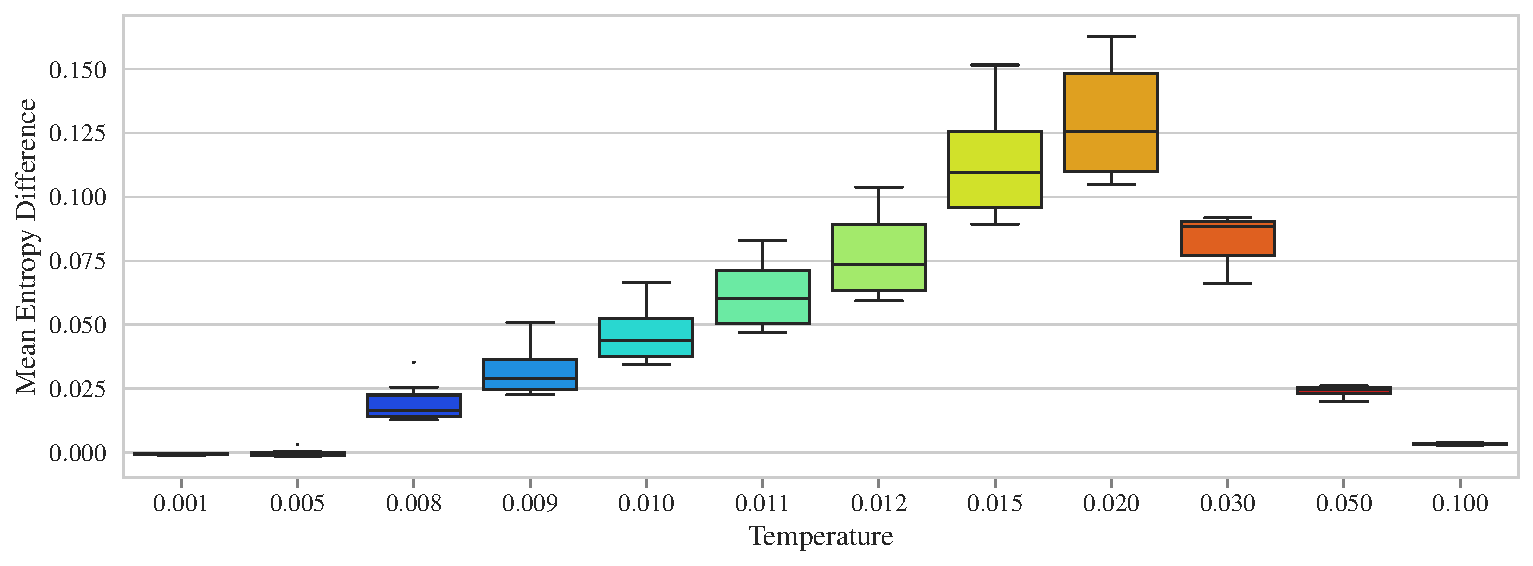
\includegraphics[width=\textwidth]{images/temperature_adversarial.pdf}
    \caption{Effect of temperature on discerning true positives from false positives.}
    \label{fig:clip-temperature-adversarial}
\end{figure}

\figref{fig:clip-temperature-adversarial} shows the effect of temperature on the adversarial performance with the difference in the mean entropies of the false positives and true positives.
Evidently, higher temperatures up to \(0.02\) are better at smoothing the reward landscape just enough to improve its adversarial performance.

\begin{figure}[H]
    \centering
    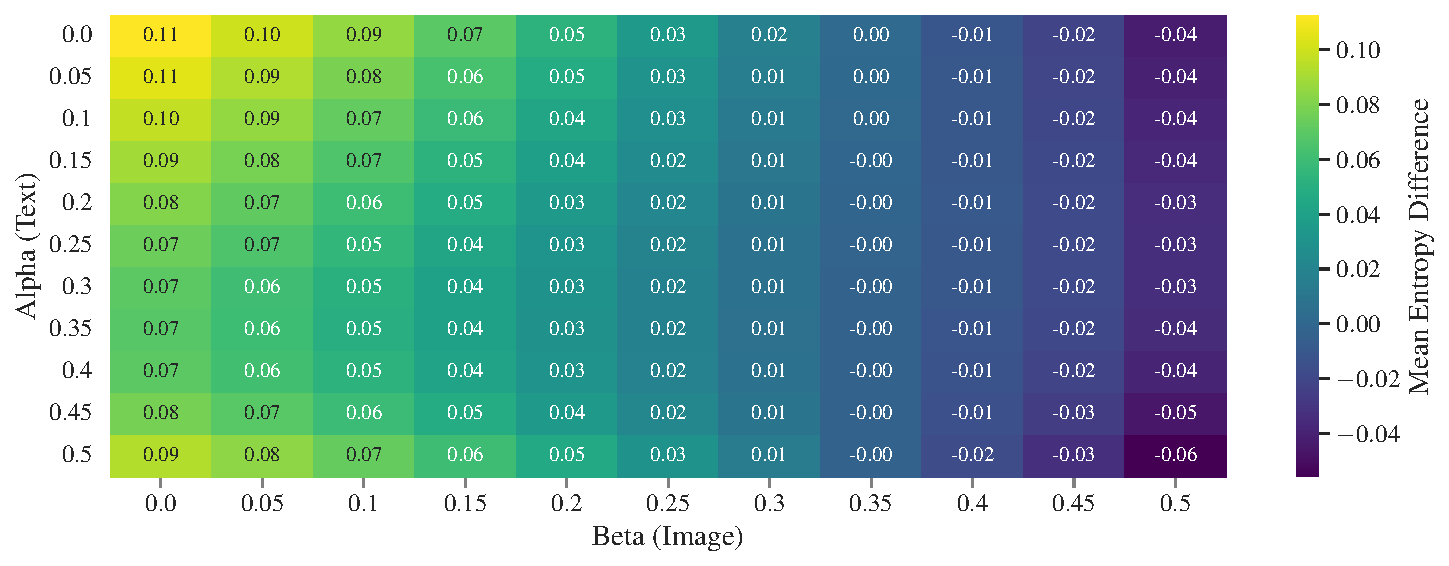
\includegraphics[width=\textwidth]{images/alpha_beta_adversarial.pdf}
    \caption{Effect of regularization strength on discerning true positives from false positives.}
    \label{fig:clip-alpha-beta-adversarial}
\end{figure}

Interestingly, the trends in the regularization strength of the text baseline (\(\alpha_{l}\)) and the image baseline (\(\beta_{i}\)) shown in \figref{fig:clip-alpha-beta-adversarial} are essentially opposite from the ones in \figref{fig:clip-alpha-beta} that showed the effect on the reward landscape.
These results are not at odds with each other, but rather complementary. 
As noted before, there is an anti-correlation between reward noise and semantic bias in random images.

An optimal choice of baseline regularization strength in the goal-based reward landscape essentially improves the path to this goal by improving the gradients to reach this desired reward.
This means that it changes the reward at states away from the goal in such a way that it is better at intimating the agent if it is close to its ultimate goal, i.e. it increases the similarity or correspondence of this state to the goal state.
This is in contrast to the adversarial performance where we desire to make this difference more pronounced.
These results are further discussed in detail in Chapter \ref{sec:discussion}.

Next, we look at the effect of different text baselines and post-suffixes on the adversarial performance.
To visualize these results, we plot the mean entropies of the false positives and true positives for different combinations of prefixes and suffixes for the text input in a 2D space.
Ideally, we would like the points (which represent prefix-suffix combinations) to live above the diagonal, i.e. the mean entropy of the false positives should be higher than the true positives.
Additionally, we plot boxplots of the difference in the mean entropies of the false positives and true positives.

\begin{figure}[H]
    \centering
    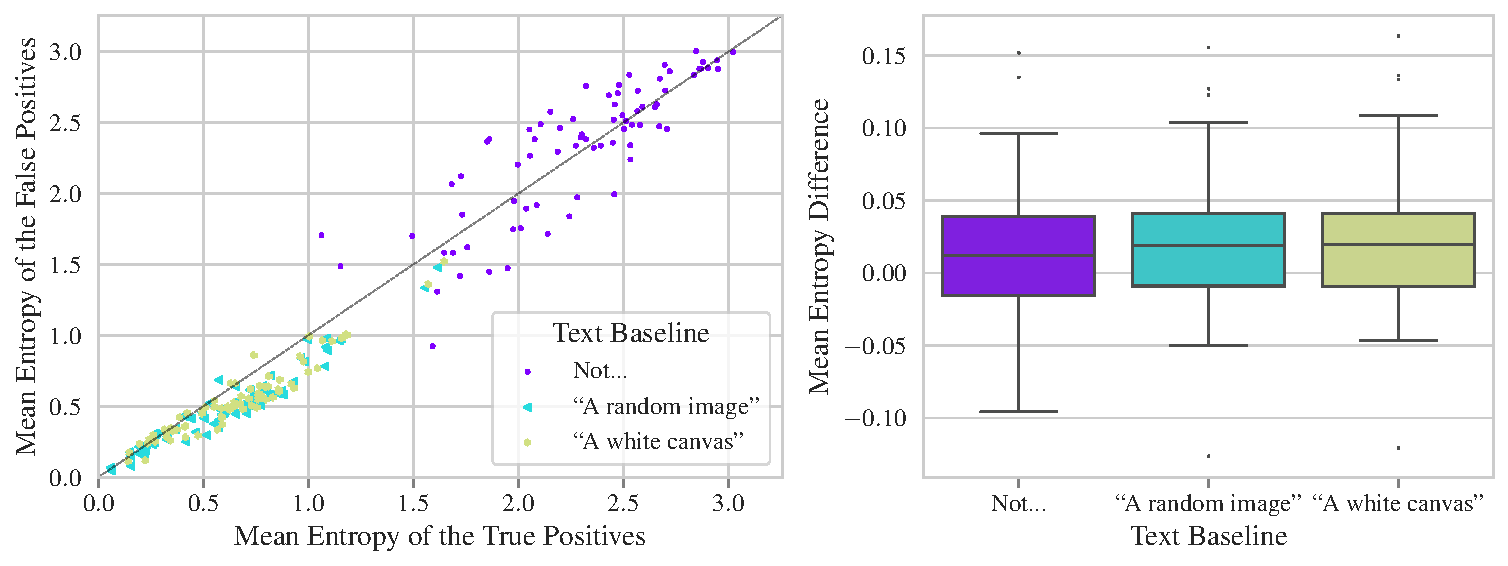
\includegraphics[width=\textwidth]{images/baseline_adversarial_2.pdf}
    \caption{Effect of different text baselines on discerning true positives from false positives.}
    \label{fig:baseline-adversarial}
\end{figure}

\figref{fig:baseline-adversarial} shows the effect of different text baselines on the adversarial performance.
Negative embeddings as we have seen before, flatten the reward landscape uniformly and as a consequence increase the entropy of the true positives as well.
This results in no performance improvement in the adversarial case.

\begin{figure}[H]
    \centering
    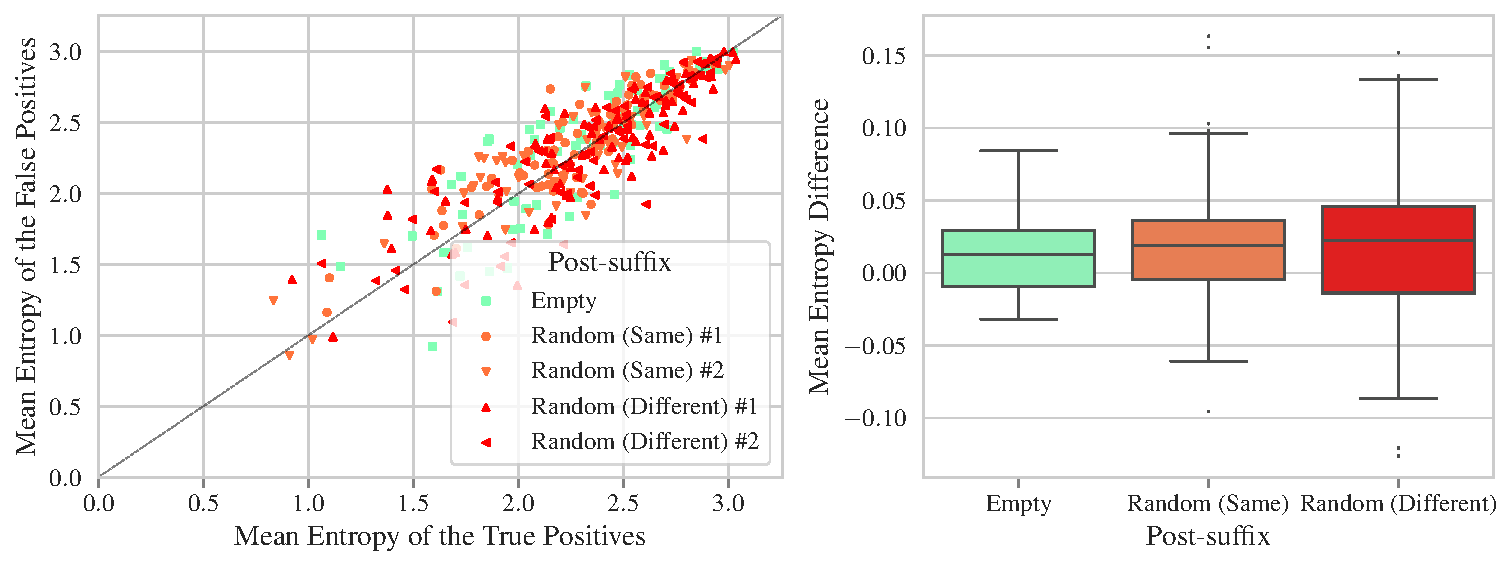
\includegraphics[width=\textwidth]{images/post-suffix_adversarial_2.pdf}
    \caption{Effect of different post-suffixes on discerning true positives from false positives.}
    \label{fig:post-suffix-adversarial}
\end{figure}

\figref{fig:post-suffix-adversarial} shows the effect of different post-suffixes on the adversarial performance.
Since the mechanism for choosing a post-suffix that works well in general is not exact, for this analysis, to ensure more exhaustive and rigorous tests, we also use different formulations of the post-suffix and consider cases such as having the same random post-suffix for the categories across every prefix-suffix combination and having a random one for each of the categories and combinations.
As before, we see no net effect in adding or omitting the post-suffix, but just a difference in variance.

% \begin{figure}[H]
%     \centering
%     \includegraphics[width=\textwidth]{images/p_subplots/rair_.pdf}
%     \includegraphics[width=\textwidth]{images/p_subplots/entropy_.pdf}
%     \includegraphics[trim=1.6cm 0cm 0cm 0cm, width=\textwidth]{images/p_subplots/distribution_.pdf}
%     \includegraphics[width=\textwidth]{images/p_subplots/snapshots_.pdf}
%     \caption{A sample rollout distribution plot.}
% \end{figure}

% \newpage
\subsection{Effect of Image Texturing}
\label{sec:image-texturing}
We also experiment with adding textures in the environment renderings
in hopes of bringing these image inputs closer to in-distribution for CLIP to improve its inference quality.
This is done by adding a constant shading to the Tangram polygons (see \figref{fig:texturing}).
Although, we do not find a significant improvement in the reward landscape with this texturing.
\figref{fig:texturing-operations} shows its effects.

\begin{figure}[H]
    \centering
    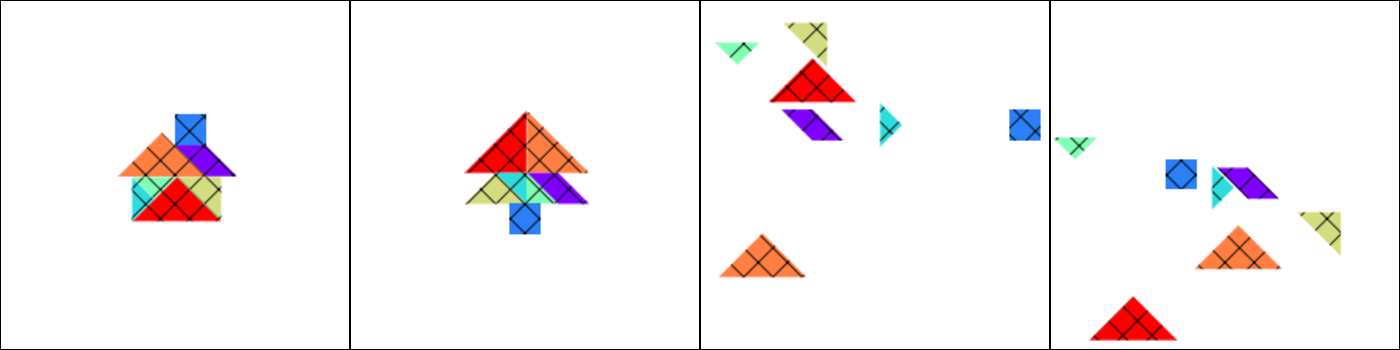
\includegraphics[width=0.8\textwidth]{images/hatched.pdf}
    \caption{Texturing in Tangram.}
    \label{fig:texturing}
\end{figure}

\subsection{Effect of Image Operations}
\label{sec:image-operations}
% Shearing and Hatching
We also test the idea of using subtle image operations like shearing before inference to denoise the CLIP signal.
We expect the true positive semantic inferences to be invariant to these operations, but the false positives to be reduced, thus reducing the noise in the reward landscape.
% This is compared together with the texturing operations in \figref{fig:texturing-operations} and \figref{fig:texturing-operations-adversarial} to study their effects on the reward landscape and the adversarial performance respectively.

As shown in \figref{fig:texturing-operations} trajectory plot, shearing the images before inference does improve the quality of the inferences slightly by smoothing the reward landscape.
It has a significant performance improvement in the adversarial case as well (\figref{fig:texturing-operations-adversarial} boxplot), but it also affects the confidence in the true positive images, thus leading to lower performance by our cumulative reward/cost metric as seen in \figref{fig:texturing-operations} cumulative reward plot.

\begin{figure}[H]
    \centering
    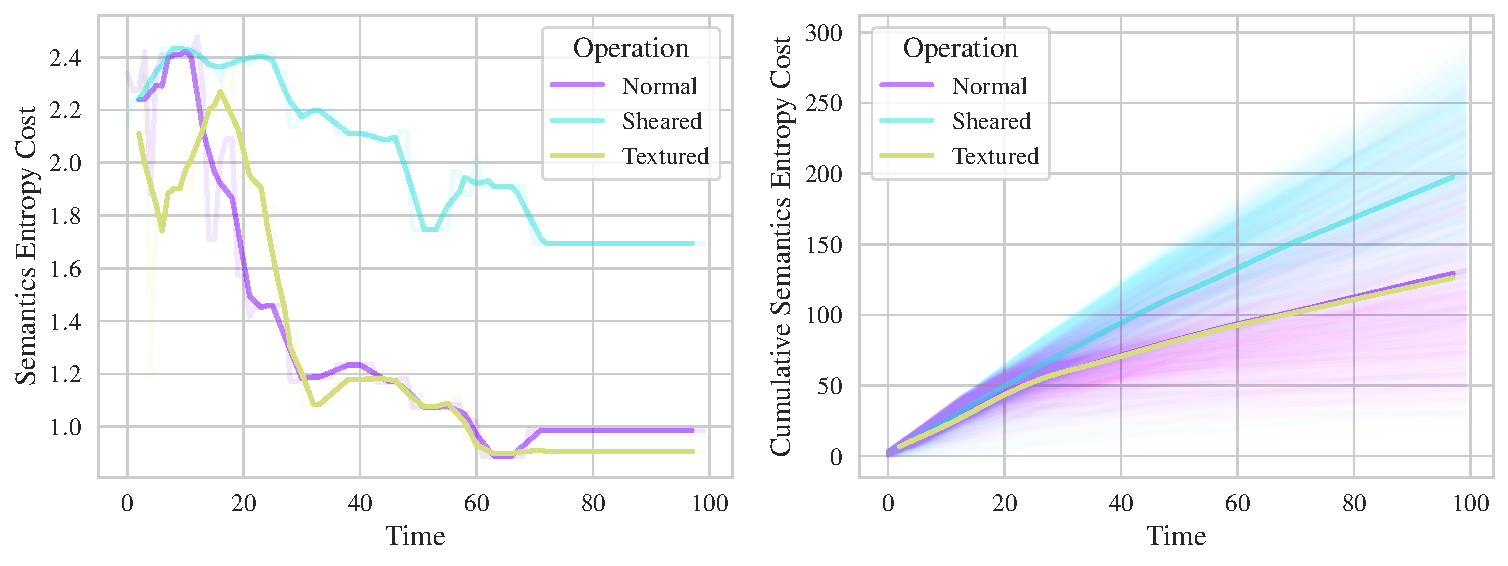
\includegraphics[width=\textwidth]{images/texturing_operations_comparison.pdf}
    \caption{Effect of texturing and image operations on semantics entropy reward trajectories.}
    \label{fig:texturing-operations}
\end{figure}

\begin{figure}[H]
    \centering
    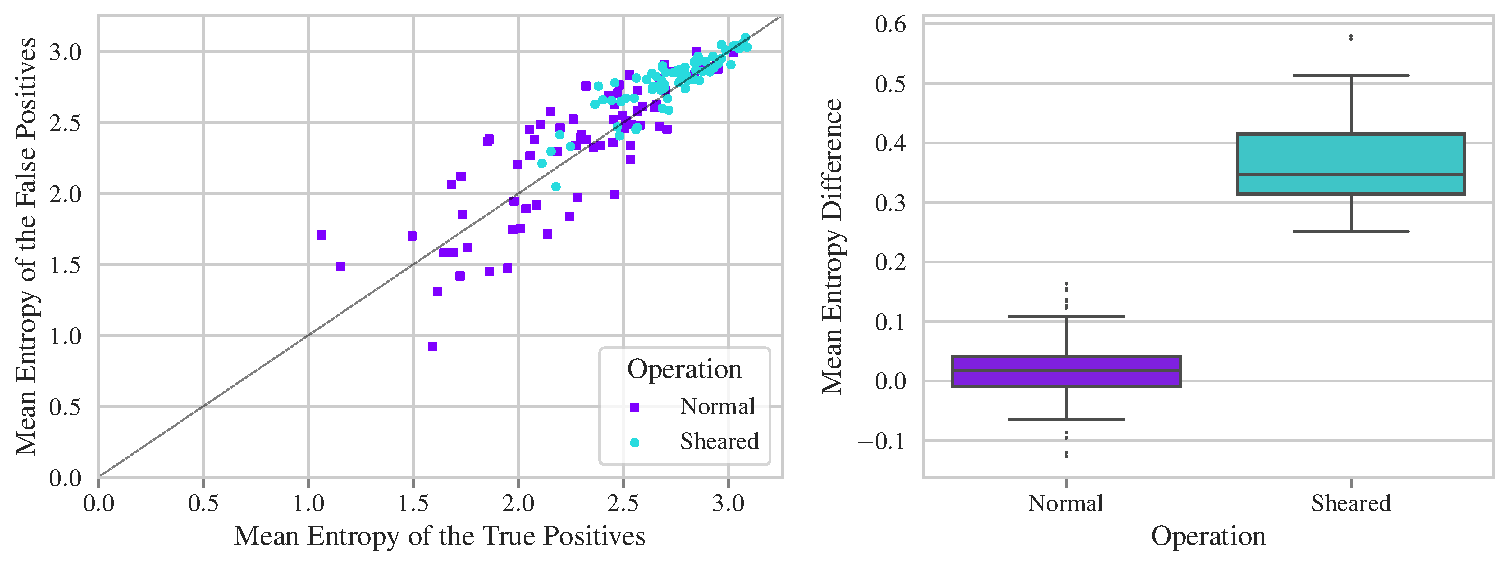
\includegraphics[width=\textwidth]{images/texturing-operations_adversarial_2.pdf}
    \caption{Effect of image operations on discerning true positives from false positives.}
    \label{fig:texturing-operations-adversarial}
\end{figure}

To additionally show the interdependence of the hyperparameters discussed above, \figref{fig:baseline_sheared_adversarial} and \figref{fig:post-suffix_sheared_adversarial} compare the adversarial performance of negative embeddings and different post-suffix patterns over sheared images respectively.

We observe that the shearing operation when used with baselines based on initial states helps improve the adversarial performance of CLIP as seen by the points gathering in the upper right corner of \figref{fig:baseline_sheared_adversarial}.

Yet, in the following sections, we do not use this method, because of the associated added computational costs of rendering, and because we realize that we can get a similar effect by tuning the baseline regularization strengths and the temperature.

\begin{figure}[H]
    \centering
    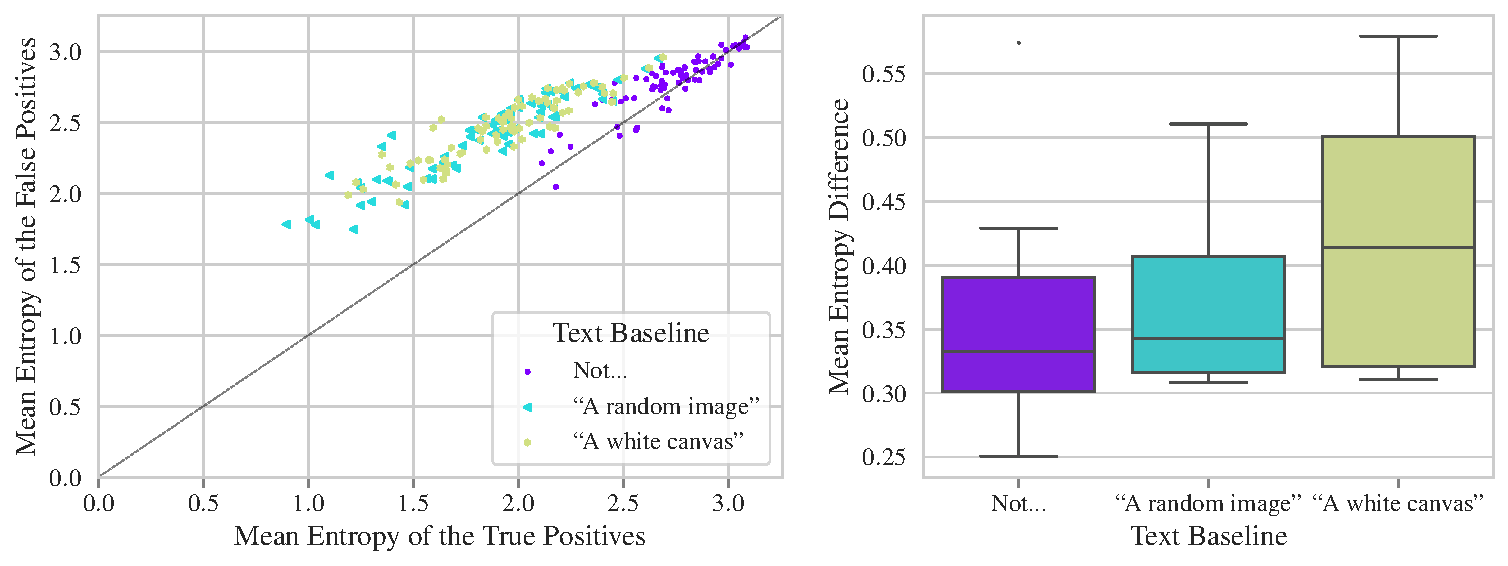
\includegraphics[width=\textwidth]{images/baseline_sheared_adversarial_2.pdf}
    \caption{Effect of different text baselines on discerning true positives from false positives with sheared images.}
    \label{fig:baseline_sheared_adversarial}
\end{figure}

The addition of post-suffixes in the sheared image case on the other hand impairs the adversarial performance, as shown in \figref{fig:post-suffix_sheared_adversarial}.
Shearing seems to surface the post-suffixes' originally intended regularization/smoothing effect which is not as visibly pronounced in the non-sheared case in the study of its effect on the reward trajectories (\figref{fig:post-suffix}).

\begin{figure}[H]
    \centering
    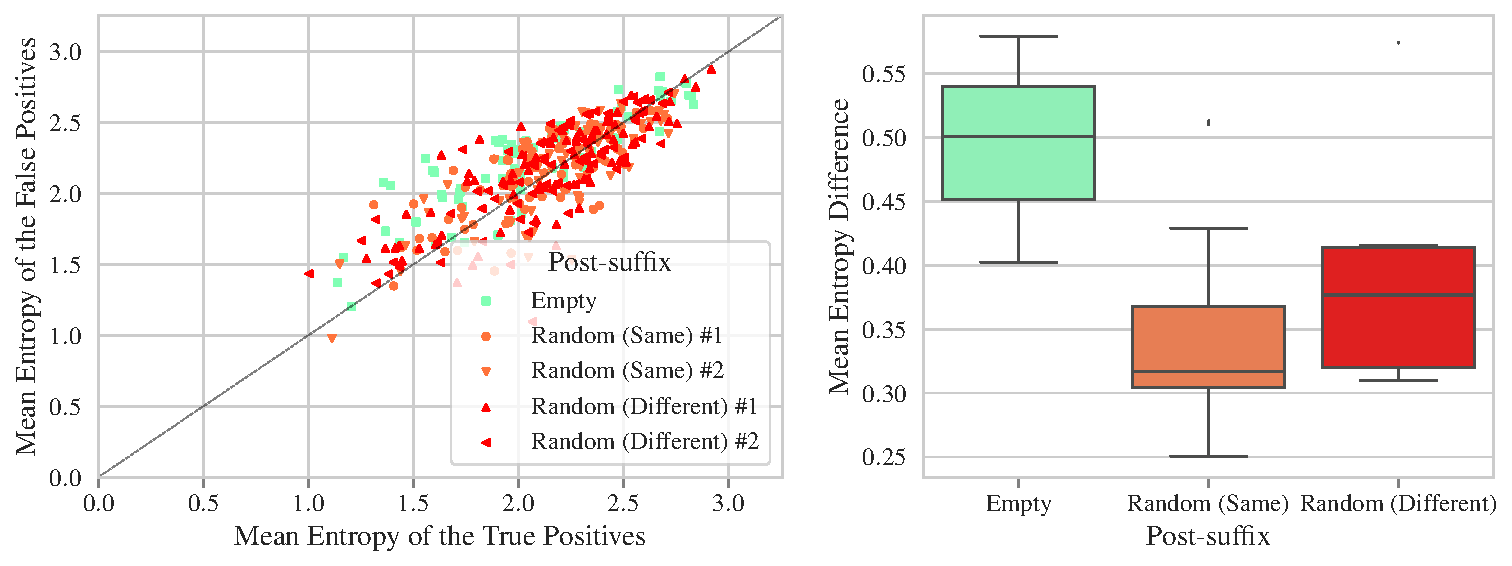
\includegraphics[width=\textwidth]{images/post-suffix_sheared_adversarial_12.pdf}
    \caption[Effect of different post-suffixes on discerning true positives from false positives with sheared images.]{Effect of different post-suffixes on discerning true positives from false positives with the sheared image. Note that the temperature used here is lower, \(\tau = 0.012\), as the points gather in the upper right corner at higher temperatures.}
    \label{fig:post-suffix_sheared_adversarial}
\end{figure}

% \newpage
\section{Simulations using the Semantics Reward}
\label{sec:simulations}
% Manual ranking and entropy ranking

Using the suitable combinations of the controller and environment hyperparameters from \secref{sec:closeness-rollouts} and insights into the regularized semantics entropy reward hyperparameters from \secref{sec:improving-rewards}, we finally run simulations (rollouts) with the semantics reward to generate creations in the environments.
We are generally able to consistently generate meaningful creations in both environments, but the quality of the creations varies slightly with the exact choice of these reward hyperparameters.

These simulations were computationally expensive and required significant time to run.
Thus, we were limited in our ability to further investigate, confirm, and fine-tune all the hyperparameters exhaustively enough. 
Consequently, we focus our analyses on the main few -- the baseline regularization strengths and the effect of the additional regularity reward, RaIR.
The results of these analyses are showcased in the following sections.
All figures plot the mean cost trajectories over the rollouts for \(10\) different random seeds for each hyperparameter combination.

While we also run enough simulations to confirm our intuitions about the other hyperparameters, only a few of our analyses use enough restarts with different random seeds to have the statistical power to make justified general claims.
These additional results are available in Chapter \ref{sec:sgw-semantics-additional} of the appendix.

To evaluate the obtained final creations, in addition to the cumulative reward, we also ask three human evaluators to manually rank all the final creations on a scale of \(1\) to \(5\) based on their apparent underlying semantic expressiveness and subjective feel/quality of the patterns.
In the following parts, shown creations (in Tangram) not particularly interesting according to these rankings are desaturated to avoid visual clutter.
Interesting creations based on these results are curated in the gallery in Chapter \ref{sec:gallery} of the appendix\footnote[1]{Animations and summary graphs of all the simulations and creations referenced in this thesis are available on \url{https://drive.google.com/drive/folders/1RdG86GLLujH3z6eDRIvdaczokpr8krnc} or \url{https://t.ly/49O3h}.}.


% B HUMAN EVALUATION
% In these cases, goal baseline regularization does not improve performance.
% Together with the results in Figure 4a, this could suggest that goal-baseline regularization is more useful for smaller CLIP models than for larger CLIP models.
% Alternatively, it is possible that the improvements to the reward model obtained by goal-baseline regularization are too small to lead to noticeable performance increases in the trained agents for the failing humanoid tasks.
% Unfortunately, a more thorough study of this was infeasible due to the cost associated with human evaluations.

% \subsection{Evaluating Regularized Entropy Reward Formulation in Goal-Conditioned Tasks}
% \label{sec:evaluating-regularized-entropy}
% % alpha_target
% % beta_image

\subsection{Effect of Regularization Strengths}
\label{sec:alpha-beta-semantics}
% Model Search
We run simulations with different regularization strengths to reconcile their effects with the results from the previous sections.
\figref{fig:alpha-beta-semantics} shows the heatmap of the mean cumulative rewards for different combinations of the regularization strengths.
% For standard deviations, please see \figref{fig:alpha_beta-semantics_std_rair}.

We find that non-zero regularization strengths (\(\alpha_{l}\) and/or \(\beta_{i}\)) do improve the performance, with mid-range values \((\alpha_{l}, \beta_{i}) = (0.3, 0.
3)\) having the best performance by these metrics.
This corroborates the results in the post hoc trajectory analysis study in \secref{sec:reg-alpha-beta}.

% alpha_beta-semantics_rair.pdf -- heatmap
\begin{figure}[H]
    \centering
    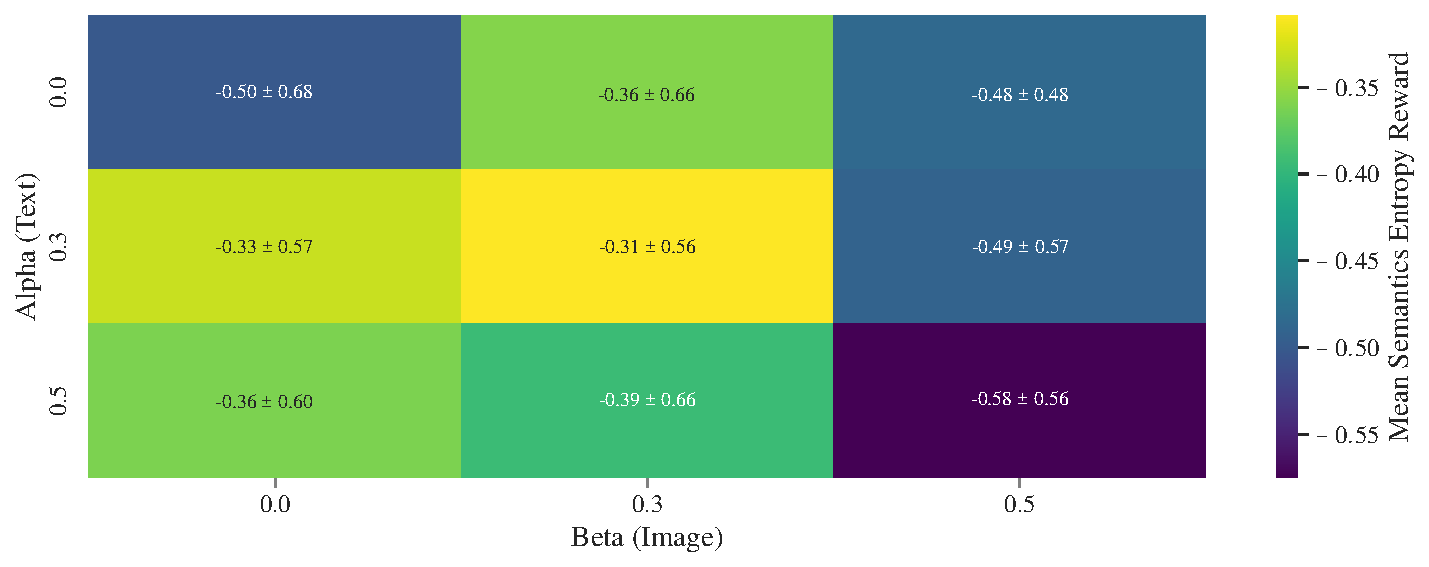
\includegraphics[width=\textwidth]{images/alpha_beta-semantics_rair_with_std.pdf}
    \caption{Performance of regularization strengths on semantics reward.}
    \label{fig:alpha-beta-semantics}
\end{figure}

\begin{figure}[H]
    \centering
    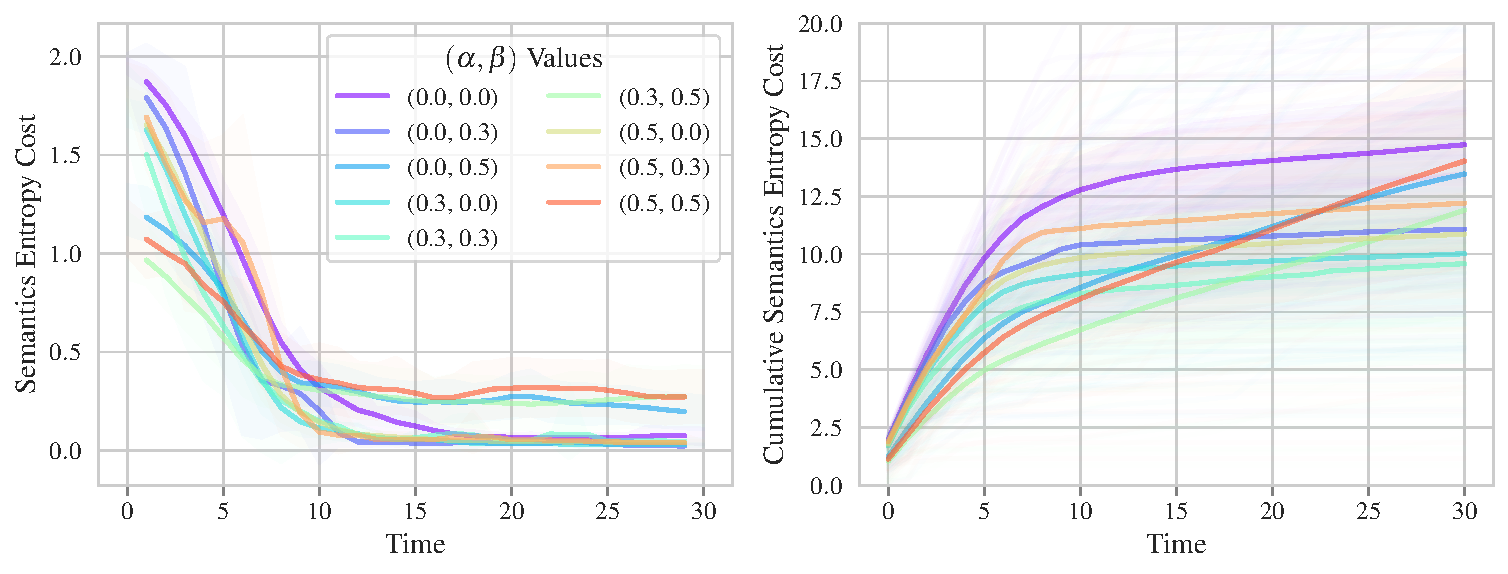
\includegraphics[width=\textwidth]{images/alpha_beta_comparison.pdf}
    \caption{Effect of regularization strengths on semantics entropy reward trajectories.}
    \label{fig:alpha-beta-trajectories}
    \vspace{12pt}
    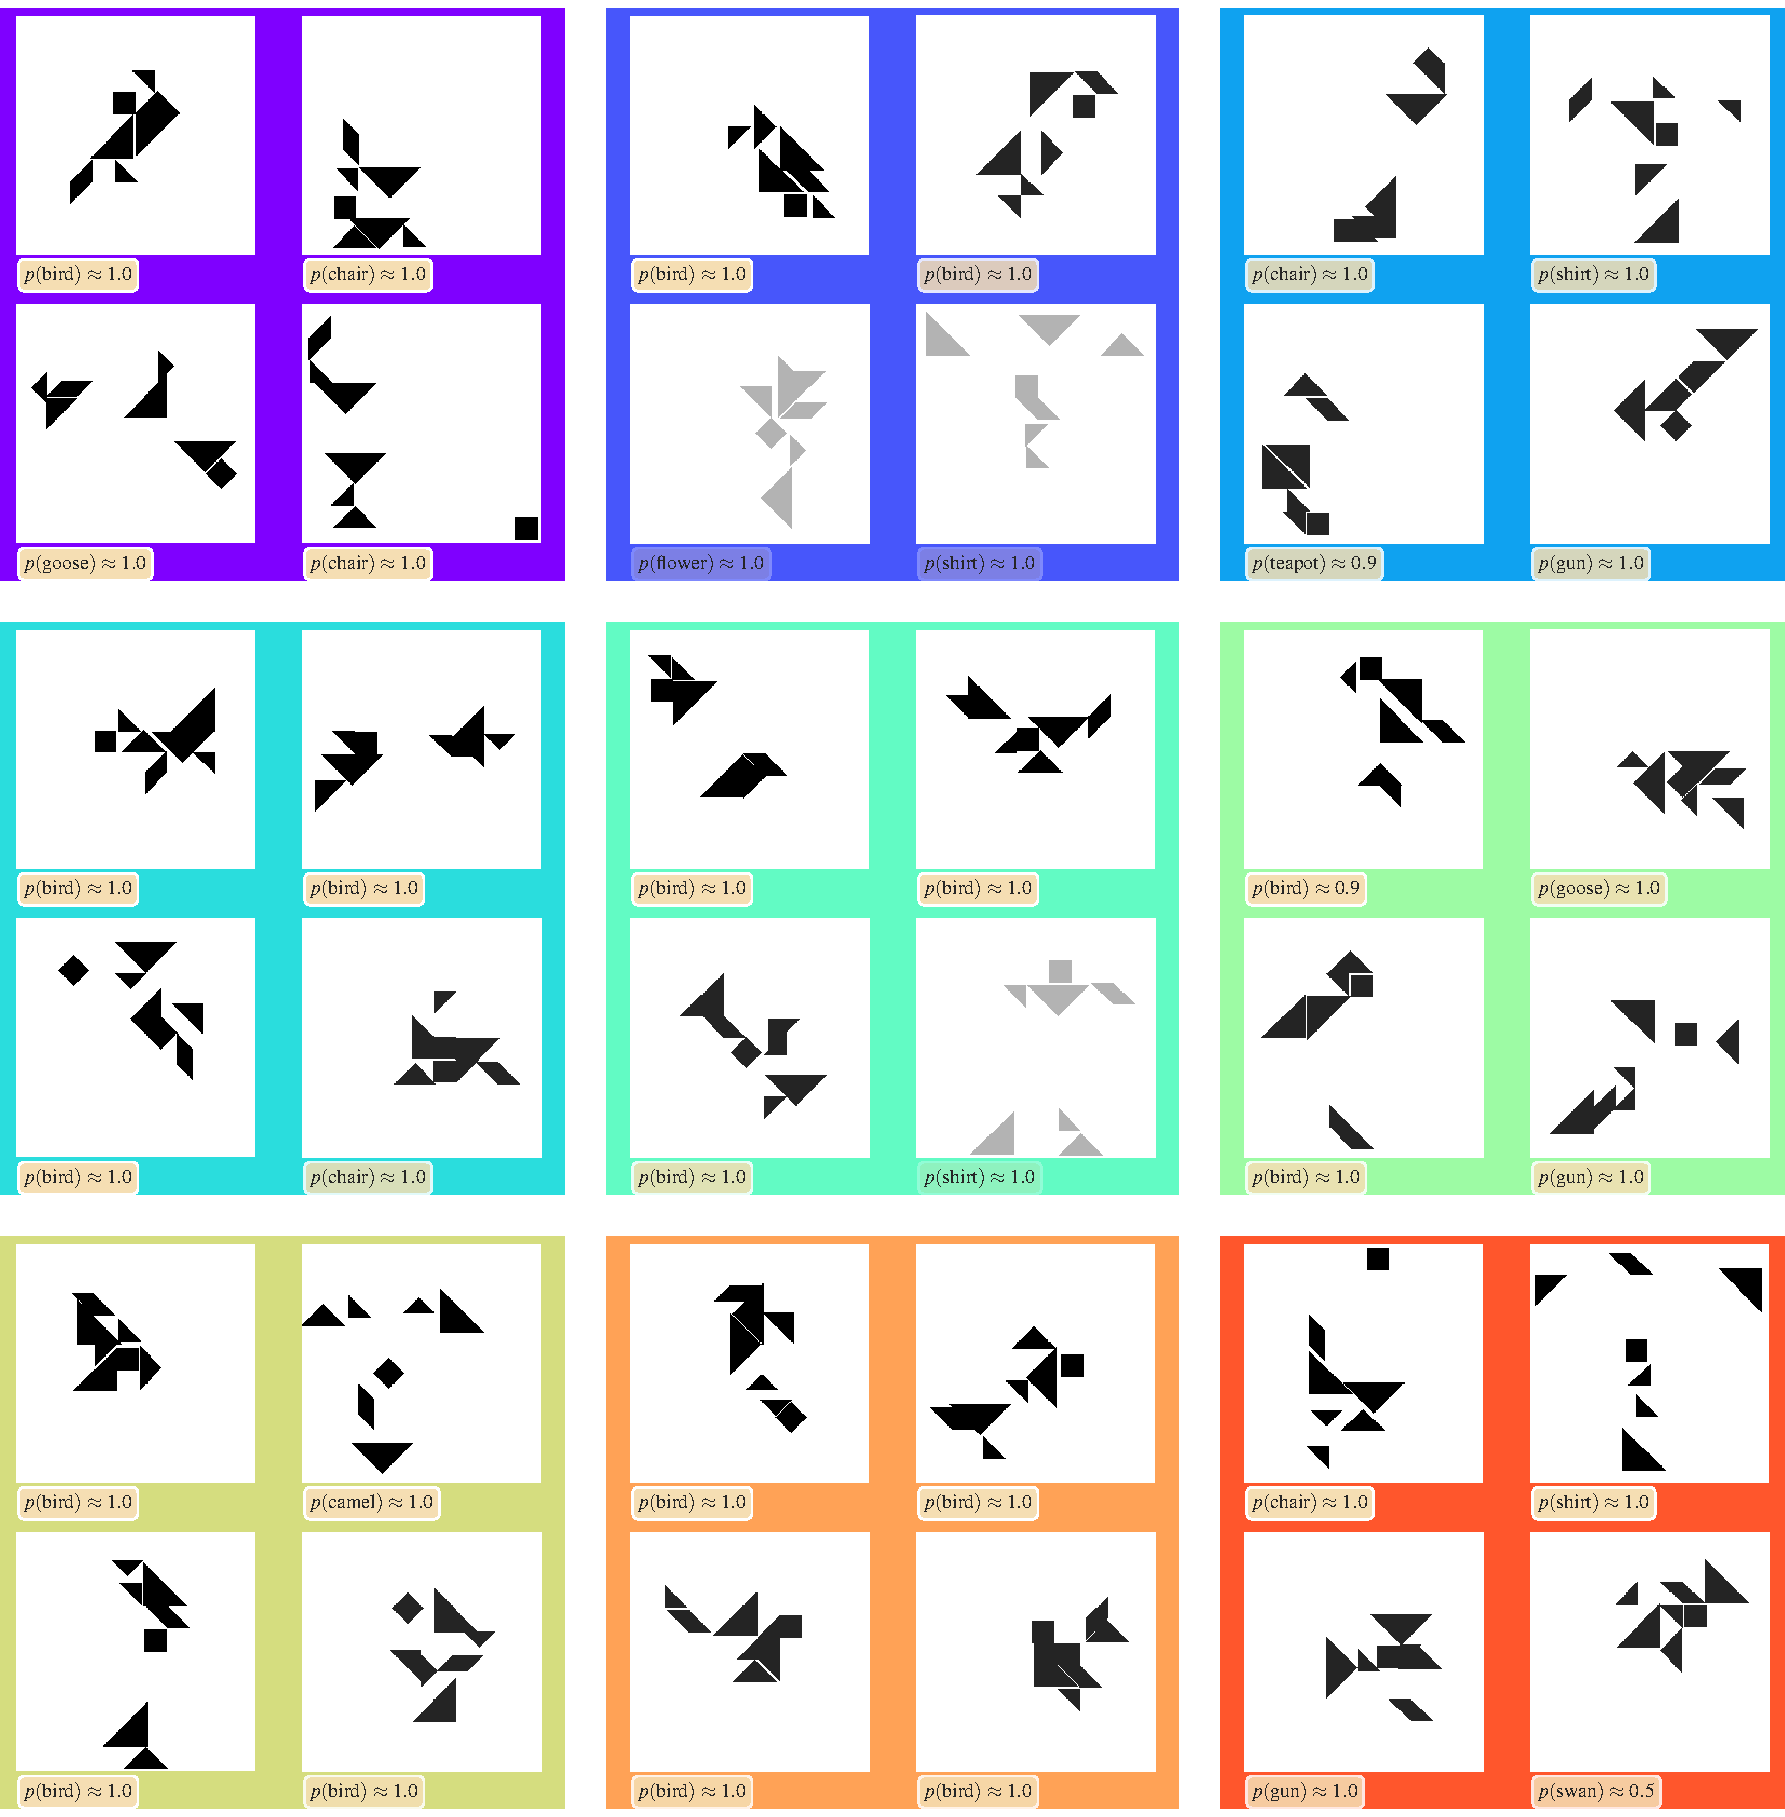
\includegraphics[width=0.8\textwidth]{images/alpha_beta_samples.pdf}
    \caption{Samples of creations with different regularization strengths.}
    \label{fig:alpha-beta-samples}
\end{figure}
\vspace{-11pt}

\figref{fig:alpha-beta-trajectories} shows the effect of regularization strengths on the semantics entropy cost trajectories and \figref{fig:alpha-beta-samples} shows some samples of the creations with different regularization strengths.
Noticeably, the three cost trajectories with high image baseline regularization strength (\(\beta_{i} = 0.5\)) are too flat and do not reach an optimal zero entropy.
At \((\alpha_{l}, \beta_{i}) = (0.5, 0.3)\) and \((0, 0.3)\), the cost trajectories seem slightly more sparse and noisy.
For the remaining combinations, \((0.5, 0)\) and \((0.3, 0)\), the trajectories are well-shaped and there is no significant difference in the performance or quality of creations.

\newpage
\subsection{Effect of RaIR}
\label{sec:effect-rair}
% compression_precision
% 1 / semantics_reward_scale

Throughout our tests, we noticed a high degree of regularity in semantic creations and high correlations between RaIR and the semantics entropy reward, suggesting a strong connection between the two.
Indeed, we find that creations simulated with RaIR are much better in some cases than without it.

Even though the performance with RaIR in Tangram is slightly worse in terms of the cumulative reward shown in \figref{fig:rair}, the creations shown in \figref{fig:rair-samples} are semantically more expressive and recognizable.
Adding structural bias using RaIR helps with grounding and coalescing the arrangements in better forms and patterns, resulting in creations that are more organized and appealing.
It is particularly helpful in the later stages of planning as the agent first quickly converges to local minima in the semantics reward landscape and then optimizes for regularity while maintaining its semantic expressiveness.
Thus RaIR helps in escaping and navigating different local minima, and in turn, leads to more meaningful creations.
This mechanism is quite apparent in the simulation summary shown in \figref{fig:sim}.

\begin{figure}[h]
    \centering
    \href{https://drive.google.com/file/d/1zhw-571KImEE4OPbpeWEA9SAKPv4r7F3}{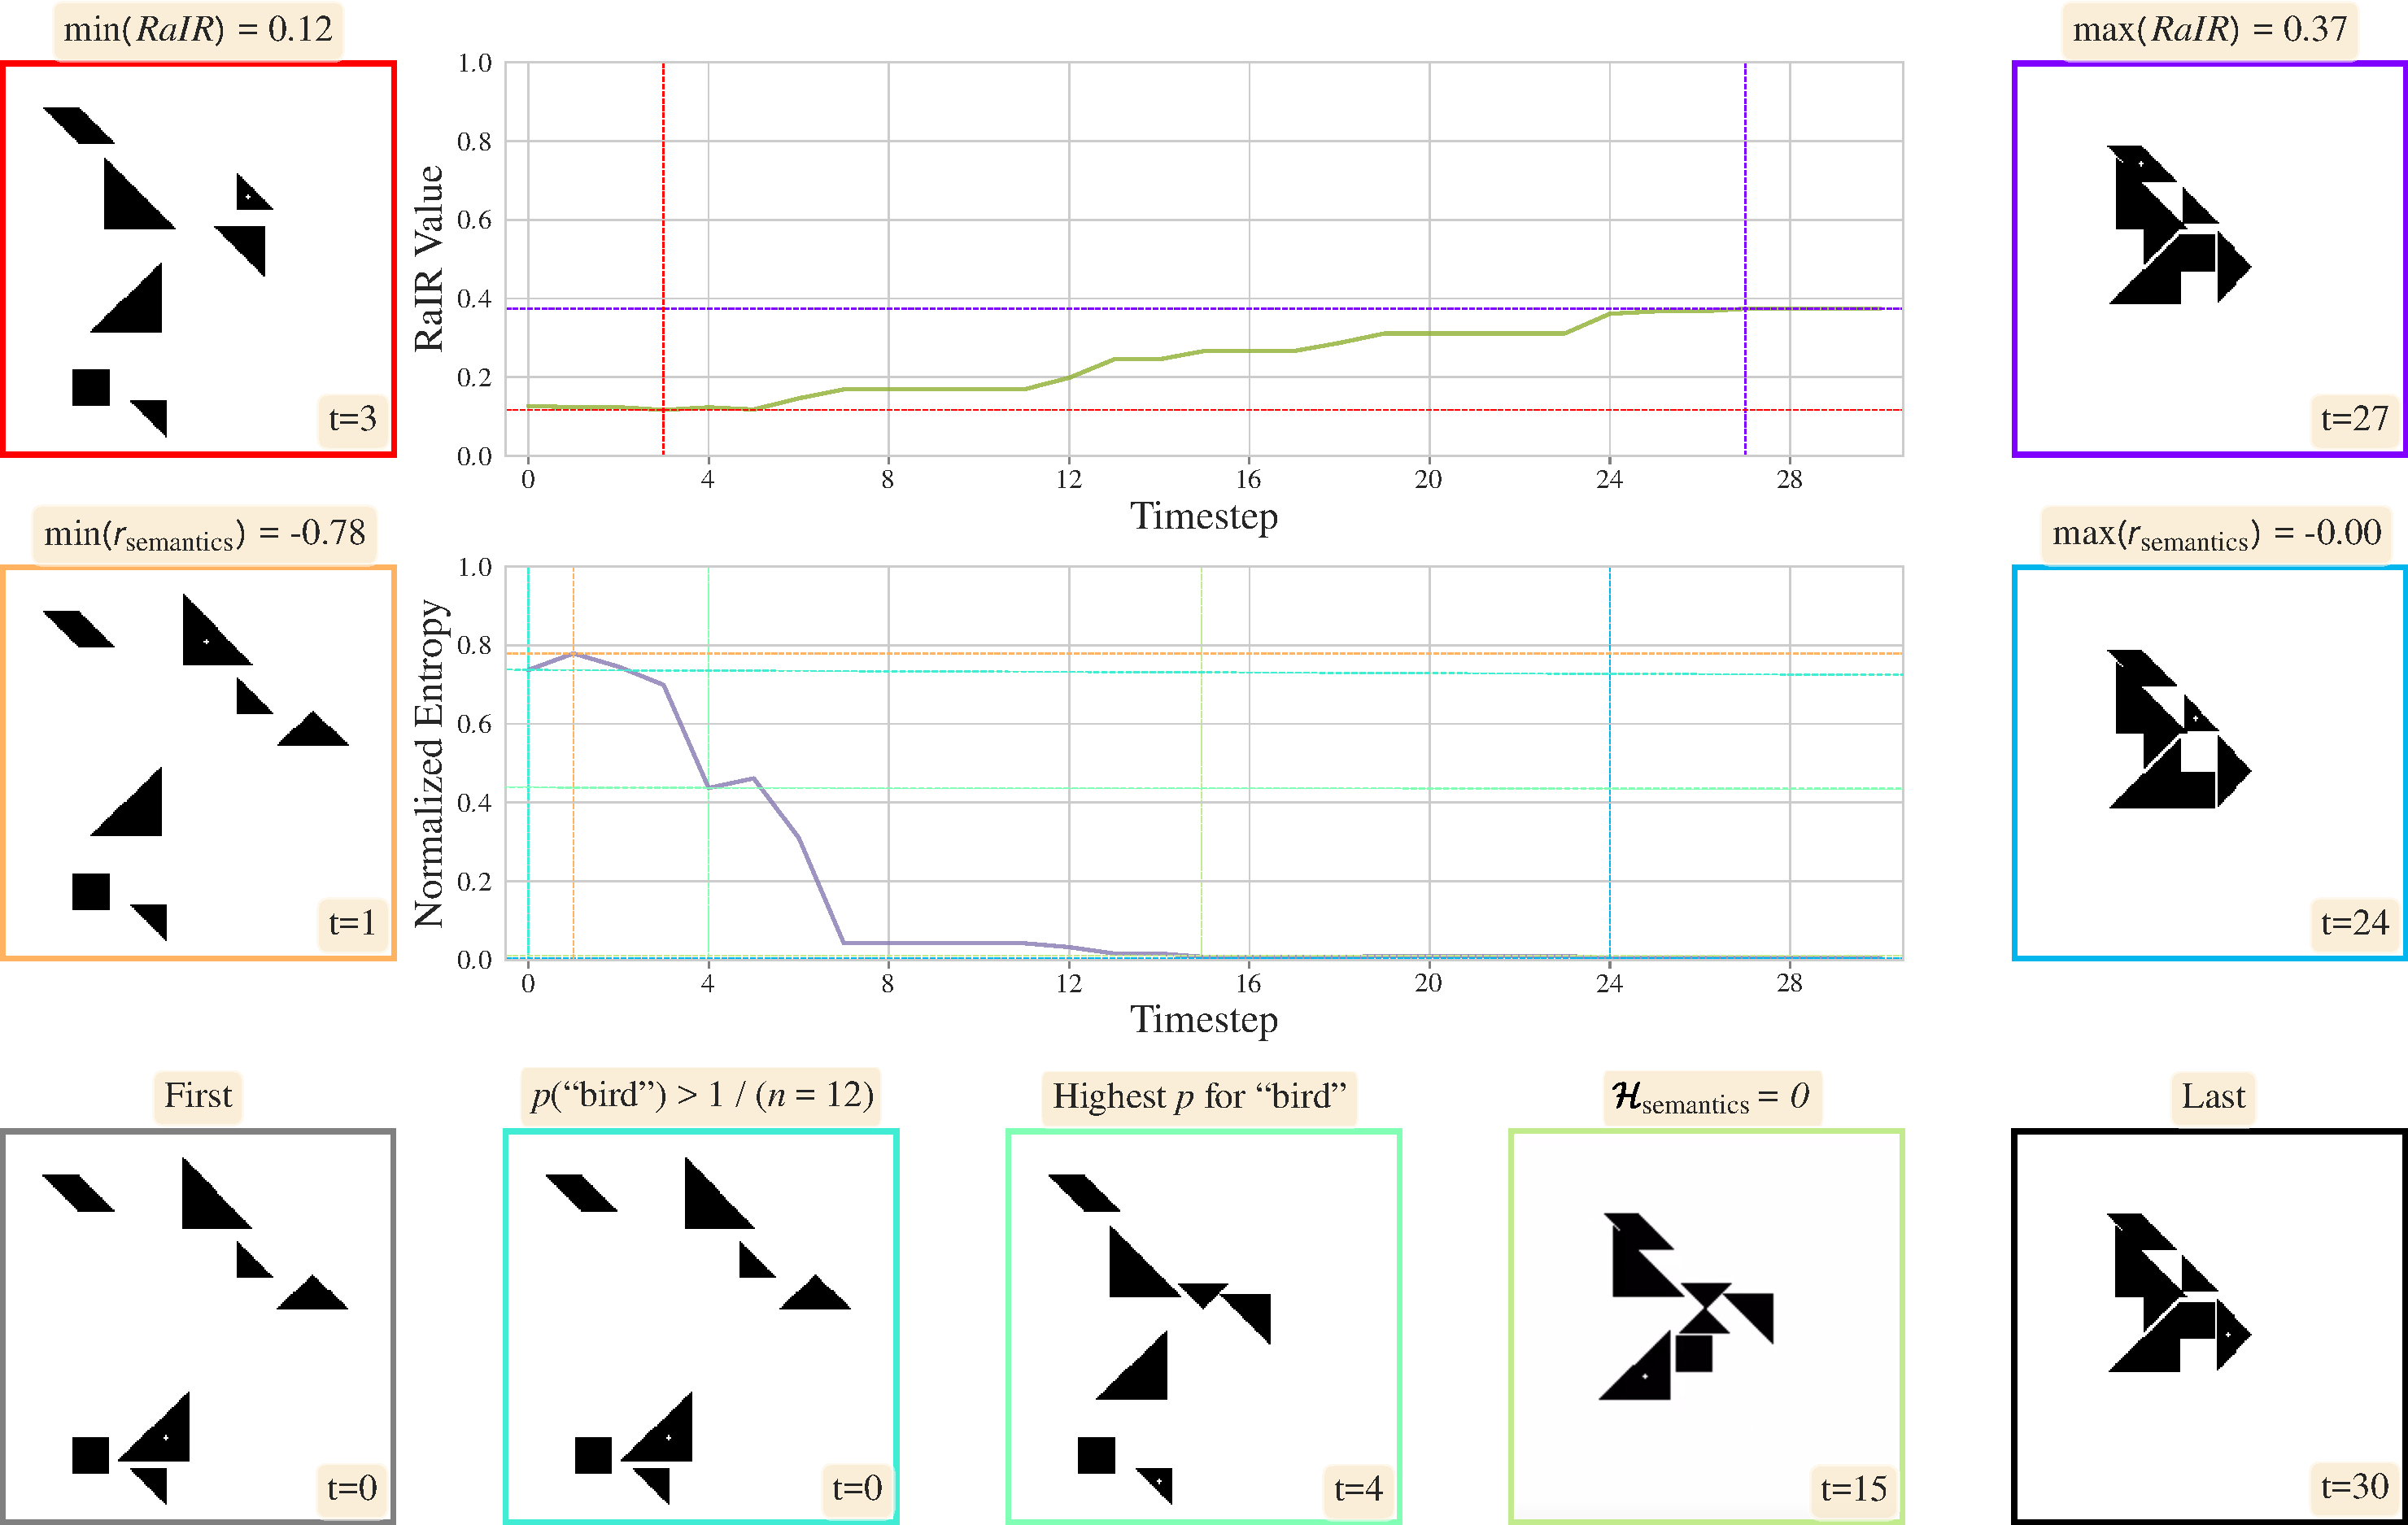
\includegraphics[width=\textwidth]{images/sim_rair_later_bird_cropped.pdf}}
    \caption[Simulation on Tangram with the complete semantics reward leading to a bird creation.]{Simulation on Tangram with the complete semantics reward leading to a bird creation. The first row shows the RaIR trajectory, the second row shows the semantics entropy cost, and the third row shows snapshots of labeled milestones across time. Notice how the semantic reward is optimized first, but does not lead to a particularly meaningful bird creation. As the regularity is optimized further, while maintaining the semantic state in the CLIP reward landscape, the creation becomes more recognizable.}
    \label{fig:sim}
\end{figure}

We also discover that the exact proportion of the weight of the RaIR to the semantics entropy reward \(\lambda\) from \eqref{eq:semantics-reward} is not as important as the presence of RaIR itself.
Although, very high values of \(\lambda\) can lead to a loss of semantic expressiveness.
Consequently, we use a value of \(\lambda = 1\) in our simulations, which results in consistent well-expressed creations.

\figref{fig:rair-sgw} and \figref{fig:rair-samples-sgw} show the effect of RaIR on the semantics reward in ShapeGridWorld, where the effect is only marginal, both in terms of the cumulative reward/cost performance, and the quality of the creations.
Although the creations are neater with RaIR, with fewer random pixels, there is no effective difference in the semantic expressiveness of the creations.
Results for many more simulations on ShapeGridWorld are given in Chapter \ref{sec:sgw-semantics-additional} of the appendix.

\begin{figure}[h]
    % rair_comparison.pdf
    \centering
    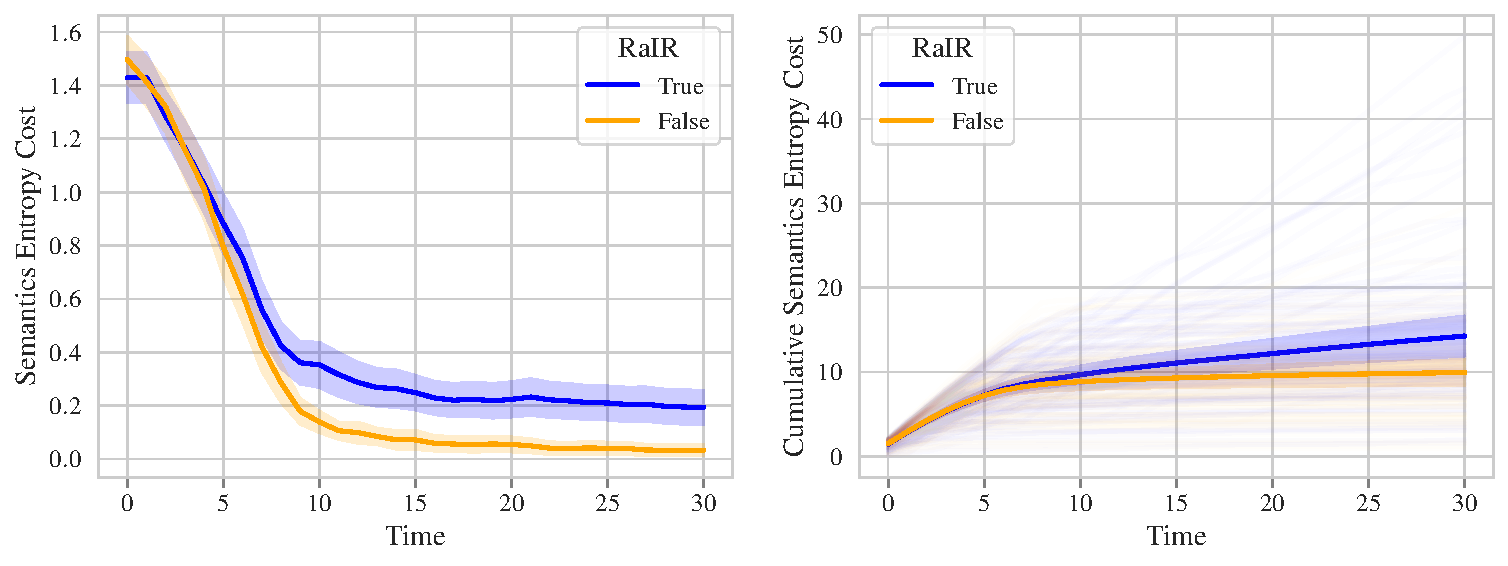
\includegraphics[width=0.99\textwidth]{images/rair_comparison.pdf}
    \caption{Effect of RaIR on semantics entropy reward in Tangram.}
    \label{fig:rair}
    \vspace{12pt}
    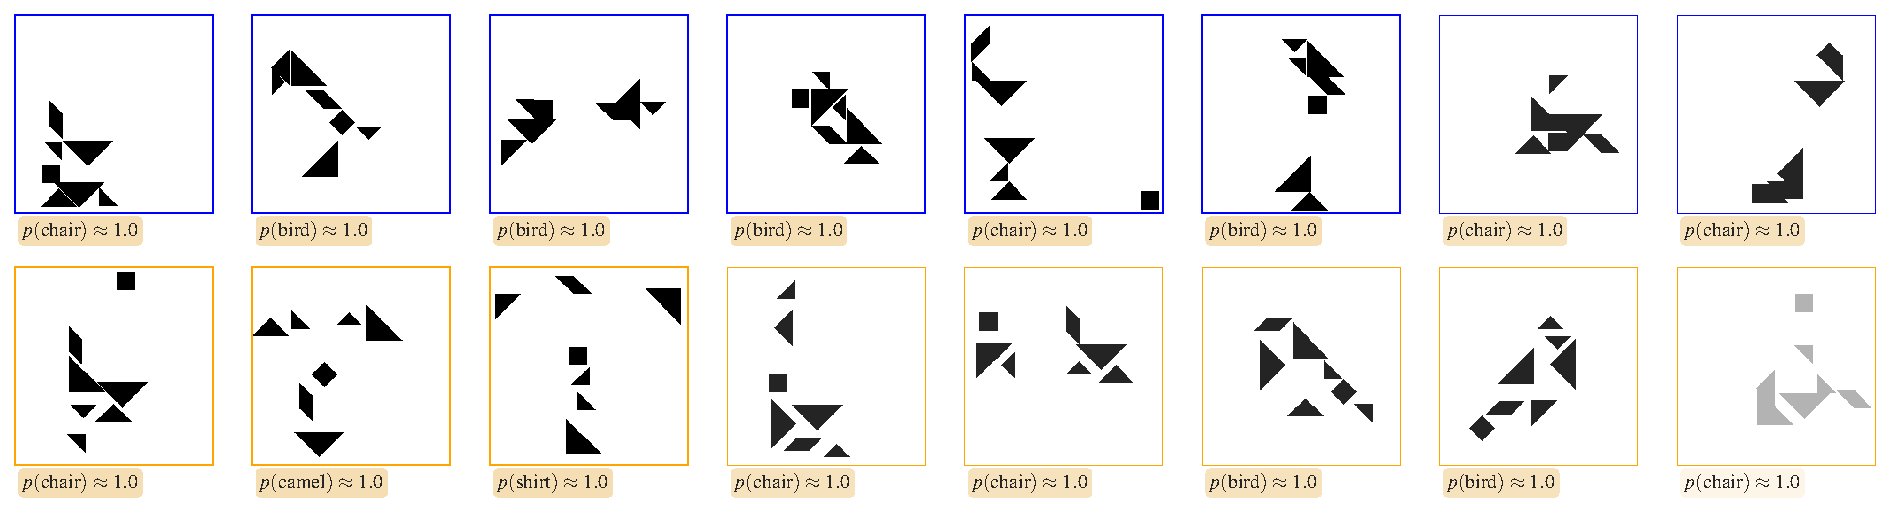
\includegraphics[width=0.99\textwidth]{images/rair_samples.pdf}
    \caption{Samples of creations with and without RaIR in Tangram.}
    \label{fig:rair-samples}
    \vspace{12pt}
    % rair_comparison_sgw_categories.pdf
    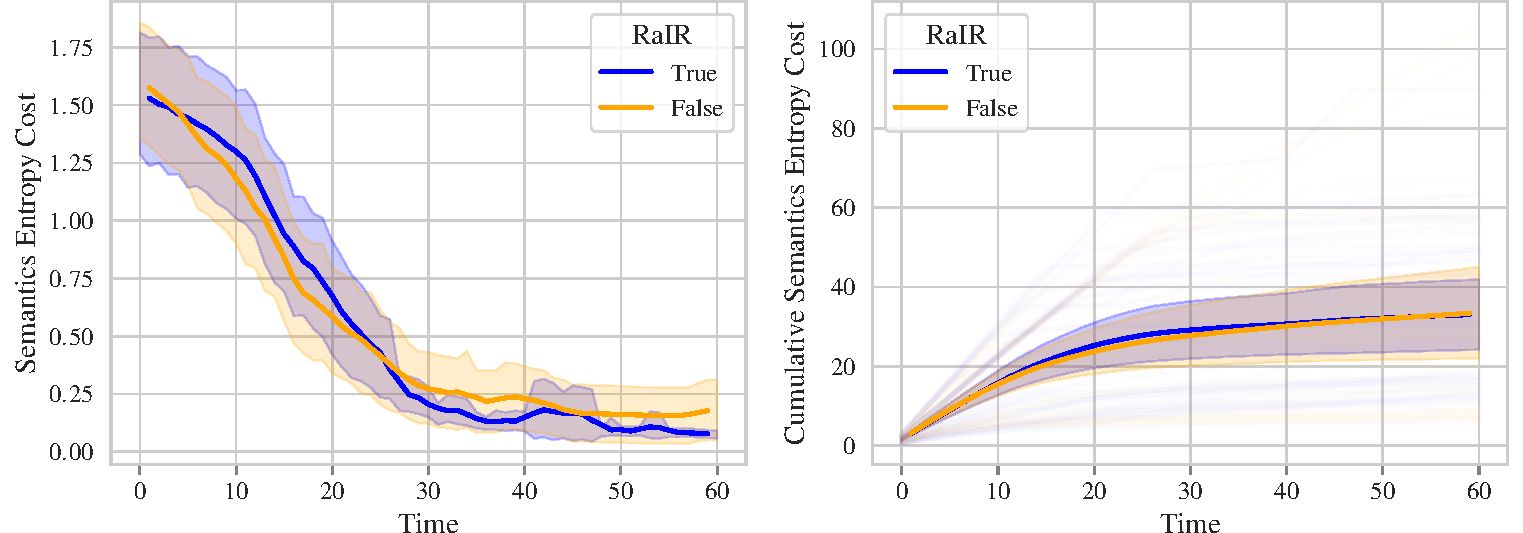
\includegraphics[width=0.99\textwidth]{images/rair_comparison_sgw_categories_cropped.pdf}
    \caption{Effect of RaIR on semantics entropy reward in ShapeGridWorld.}
    \label{fig:rair-sgw}
    \vspace{12pt}
    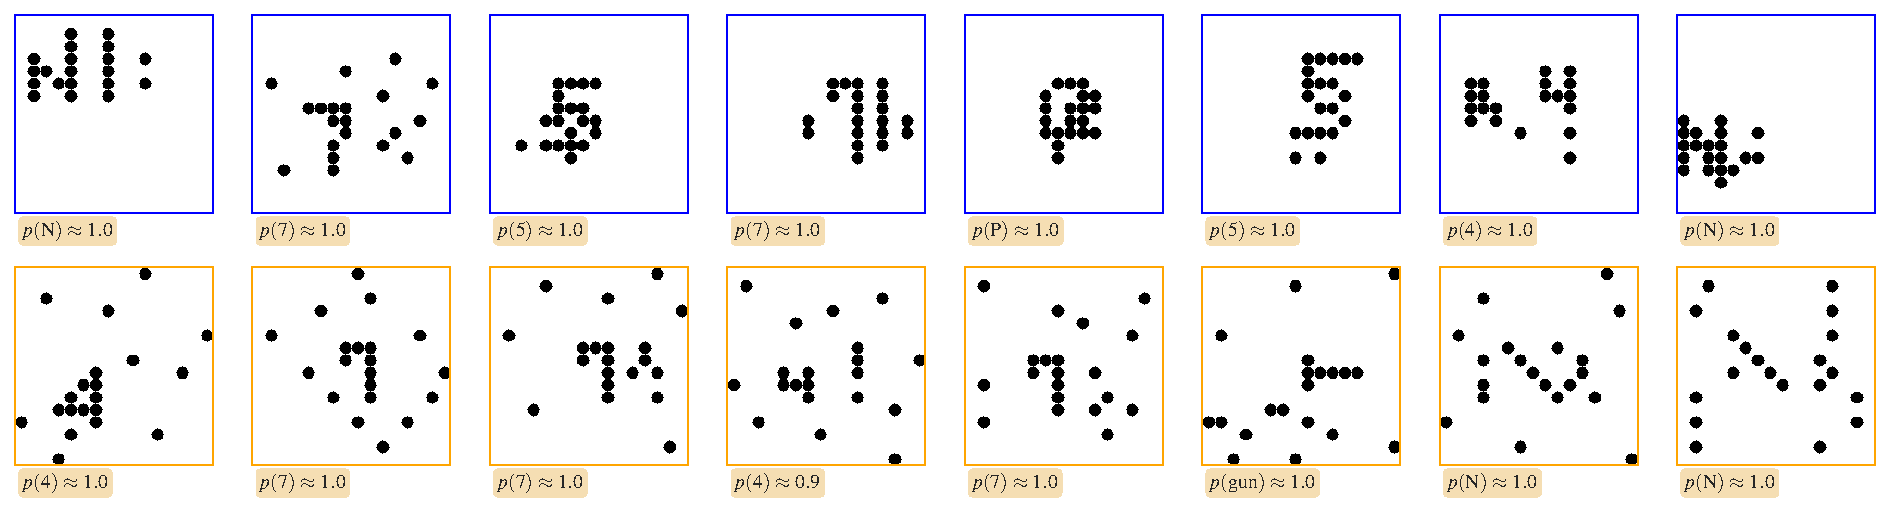
\includegraphics[width=0.99\textwidth]{images/rair_samples_sgw_categories.pdf}
    \caption[Samples of creations with and without RaIR in ShapeGridWorld.]{Samples of creations with and without RaIR in ShapeGridWorld. % Using the \texttt{best} aggregation function.
    }
    \label{fig:rair-samples-sgw}
\end{figure}

% \subsection{Final Simulations on ShapeGridWorld}
% \label{sec:sgw-semantics}

% While we were consistently able to get good creations on Tangram, the results on ShapeGridWorld due to the many degrees of freedom were more varied.

% We ran final simulations on ShapeGridWorld with the best hyperparameters from the previous analyses.
% \figref{fig:sgw-trajectories} shows the effect of regularization strengths on the semantics entropy reward trajectories.

